%%%%%%%%%%%%%%%%%%%%%%%%%%%%%%%%%%%%%%%%%%%%%%%%%%%%%%%%%%%%%%%%%%%%%%%%%%%%%%%%%%%%%%%%%%%%%%%
%%%%%%%%%%%%%%%%%%%%%%%%%%%%%%%%%%%%%%%%%%%%%%%%%%%%%%%%%%%%%%%%%%%%%%%%%%%%%%%%%%%%%%%%%%%%%%%
%% LaTeX-Beamer template for KIT design
%% by Erik Burger, Christian Hammer
%% title picture by Klaus Krogmann
%%
%% version 2.1
%%
%% mostly compatible to KIT corporate design v2.0
%% http://intranet.kit.edu/gestaltungsrichtlinien.php
%%
%% Problems, bugs and comments to
%% burger@kit.edu
%%
%%
%% Modified: 30.1.2013, Schwall
\PassOptionsToPackage{table}{xcolor}
\documentclass[16pt]{beamer}

% Fasten the compilation process 
\newif\ifmoti
%\motitrue
\motifalse

\newif\ifinter
%\intertrue
\interfalse

%\setbeamertemplate{note page}[plain]
%\setbeameroption{show only notes}
%\usepackage{pgfpages}
%\setbeameroption{show notes}
%\setbeameroption{show notes on second screen=right}

%% SLIDE FORMAT
\usepackage{templates/beamerthemekit}
%\usepackage{ngerman}
\usepackage[ngerman]{babel}
%\usepackage[T1]{fontenc}
%\usepackage[utf8]{inputenc} % Für Linux

%\usepackage{color}
%\usepackage[table]{xcolor} 
%\usepackage{multirow} 


%% german time format (e.g 30.1.2013)
\usepackage{datetime}
\newdateformat{germandate}{\THEDAY.\THEMONTH.\THEYEAR}
\newdateformat{americandate}{\THEMONTH/\THEDAY/\THEYEAR}

% use these packages for PCM symbols and UML classes
\usepackage{templates/tikzkit}
\usepackage{templates/tikzuml}

% My Packages:
\usepackage{siunitx}
\sisetup{locale = DE}%, 
%		 range-phrase={bis},  % muss trotzdem nochmal definiert werden!!
%		 range-units = single       % Einheiten bei Fehlern und Range nicht wiederholen}

\usepackage{tikz}
\usetikzlibrary{fadings,shapes,arrows,shadows,decorations.pathreplacing}
%\usetikzlibrary{angles,quotes,babel,shapes,snakes,calendar,matrix,backgrounds,folding,arrows,decorations.pathmorphing,trees,arrows.meta,calc,intersections,positioning,decorations.markings}
%\tikzset{>=latex} % Latex style set
\usepackage{makecell}
%\usepackage{booktabs} % professionelle tabellen (\toprule, \midrule, ...)

%% My own code: 
%%%%%%%%%%%%%%%%%%%%%%%%%
% eigene Kommandes
%

\usepackage{trfsigns}

% transform as symbol
\def\transform{\; \laplace \;}
\def\Transform{\; \Laplace \;}

\newcommand{\vTransform}[1][]{\mbox{\setlength{\unitlength}{0.1em}%
		\begin{picture}(10,20)%
		\put(3,2){\circle{4}}%
		\put(3,4){\line(0,1){12}}%
		\put(3,18){\circle*{4}}%
		\put(10,7){#1}
		\end{picture}%
	}%
}%

\newcommand{\vtransform}[1][]{\mbox{\setlength{\unitlength}{0.1em}%
		\begin{picture}(10,20)%
		\put(3,2){\circle*{4}}%
		\put(3,4){\line(0,1){12}}%
		\put(3,18){\circle{4}}%
		\put(10,7){#1}
		\end{picture}%
	}%
}%     


% Schlagwort
\newcommand\schlagwort[1]{\textbf{\textcolor{kit-green100}{#1}}}

% Farben f�r Boxen
\setbeamercolor{color_lower}{fg=black,bg=kit-green15}
\setbeamercolor{color_upper}{fg=black,bg=kit-green70}
%\footnotesize\tiny

%Zahlenk�rper
\def\rz{\ifmmode{\mathbb{R}}%
    \else{\hbox{$\mathbb{R}$}}\fi} 
\def\nz{\ifmmode{\mathbb{N}}%
    \else{\hbox{$\mathbb{N}$}}\fi} 
\def\gz{\ifmmode{\mathbb{Z}}%
   \else{\hbox{$\mathbb{Z}$}}\fi} 
\def\cz{\ifmmode{\mathbb{C}}
    \else{\hbox{$\mathbb{C}$}}\fi}%
\def\qz{\ifmmode{\mathbb{Q}}%
    \else{\hbox{$\mathbb{Q}$}}\fi}%   
\def\K{\ifmmode{\mathbb{K}}%
    \else{\hbox{$\mathbb{K}$}}\fi}%  

% Erwartungswert
\def\Er{\ifmmode{\mathbb{E}}%
    \else{\hbox{$\mathbb{E}$}}\fi}%  

% Real- und Imagin�rteil
\def\real{{\text{Re}}}
\def\imag{{\text{Im}}}

% simple implication within the text
%\def\thus{{$\implies$}}
\def\thus{\relax
	\ifmmode
		\implies
	\else
		$\implies$
	\fi}

%Mengen durch kaligraphische Buchstaben
\def\setS{\mathcal{S}}
\def\setP{\mathcal{P}}
\def\setX{\mathcal{X}}
\def\setY{\mathcal{Y}}
\def\setZ{\mathcal{Z}}
\def\setC{\mathcal{C}}
\def\defl{:=}
\def\Pr{P}

% Befehl zur Ausrichtung der itemize-Bullets in Columns; erfordert in den Frames ein \AdjustMargins
\makeatletter
\newcommand*{\AdjustMargins}{%
    \setlength{\beamer@rightmargin}{0em}%
    \setlength{\beamer@leftmargin}{0em}%
}
\makeatother

% Declare operators
\DeclareMathOperator*{\mini}{min}
\DeclareMathOperator*{\argmin}{arg\,min}
\DeclareMathOperator*{\maxi}{max}


% colored small box representing end of a proof
\def\endofproof{
	\ifmmode
		\text{\hfill} \textcolor{KITgreen}{\rule{2mm}{2mm}}
	\else
		$\hfill \textcolor{KITgreen}{\rule{2mm}{2mm}}$
	\fi}

% colored box for definition and theorems
\newcommand\theobox[2]{
	\begin{center}
	\begin{beamerboxesrounded}
	[upper=color_upper,lower=color_lower,shadow=true]
	{\textcolor{white}{\textbf{#1}}}
	#2
	\end{beamerboxesrounded}
	\end{center}
}


% Boxed equation 
\newcommand{\eqbox}[1]{
\begin{center}
\setlength{\fboxsep}{2mm}
\setlength{\fboxrule}{0.3mm}
\fcolorbox{kit-green100}{white}
%{\parbox{.9\linewidth \fboxsep \fboxrule}{
{\parbox{.9\linewidth }{
\bigskip
#1
\bigskip
}}
\end{center}
}


% new definition of for a boxed equation 
\newcommand{\eqboxed}[1]{
\begin{center}
\fcolorbox{kit-green100}{white}{
$#1$
}
\end{center}}


% Literature as intended
\setbeamertemplate{bibliography item}[text]


% Befehl zur Erh�hung der Section number
\makeatletter
\newcommand{\setnextsection}[1]{%
	\setcounter{section}{\numexpr#1-1\relax}%
	\beamer@tocsectionnumber=\numexpr#1-1\relax\space}
\makeatother

	
% Direktes Fu�note bauen und zitieren
\def\footcit#1{\footnote{\scriptsize Nach \cite{#1}}}


% Konstruktion einer �bersicht bei jedem Aufruf von \subsection
% Nur die aktuelle ist schwarz, alle anderen sind grau
\AtBeginSubsection[]
{
  \begin{frame}[t] 
       \frametitle{�bersicht}
       \tableofcontents[currentsection,currentsubsection]
  \end{frame}
}



%%%%%%%%%%%%%%%%%%%%%%%%%%%%%%%%%%%%%%%%%%%%%%%%%%%%%%
% Private "`Testsektion"'
\setbeamercolor{color_lower}{fg=KITblack,bg=kit-green15}
\setbeamercolor{color_upper}{fg=KITblack,bg=kit-green70}
\setbeamertemplate{navigation symbols}{}

\def\colorize<#1>{%
	\temporal<#1>{\color{KITblack}}{\color{KITblack30}}{\color{KITblack}}}

\definecolor{KITgreen}{rgb}{0,.59,.51}
\definecolor{KITblack}{rgb}{0,0,0}


% Fu�note anpassen, so dass es nicht mit dem Footer �berschneidet
\addtobeamertemplate{footnote}{\vspace{-6pt}\advance\hsize-0.5cm}{\vspace{6pt}}
\renewcommand*{\footnoterule}{\kern -3pt \hrule width 1in \kern 8.6pt}
\footnotesize\scriptsize



\newcommand\FourQuad[4]{%
	\begin{minipage}[b][.35\textheight][t]{.47\textwidth}#1\end{minipage}\hfill%
	\begin{minipage}[b][.35\textheight][t]{.47\textwidth}#2\end{minipage}\\[1em]
	\begin{minipage}[b][.35\textheight][t]{.47\textwidth}#3\end{minipage}\hfill
	\begin{minipage}[b][.35\textheight][t]{.47\textwidth}#4\end{minipage}%
}

%%%%%%%%%%%%%%%%%%%%%%%%%%%%%%%%%%%%%%%%%%%%%%%%%%%%%%%%%%%%%%%%%%%%%
%% Code to spread out slides contents using \stretchy command: (inserted by Jo)
\let\svpar\par
\let\svitemize\itemize
\let\svenditemize\enditemize
\let\svitem\item
\def\newpar{\def\par{\svpar\vfill}}
\def\newitem{\def\item{\vfill\svitem}}
\let\svcenter\center
\let\svendcenter\endcenter
\let\svcolumn\column
\let\svendcolumn\endcolumn
\newlength\columnskip
\columnskip 0pt
\def\newcolumn{%
	\renewenvironment{column}[2]%
	{\svcolumn{##1}\setlength{\parskip}{\columnskip}##2}%
	{\svendcolumn\vspace{\columnskip}}}

\newcommand\stretchy{\only<1>{%
		\newpar\def\item{\svitem\newitem}%
		\renewenvironment{itemize}{\svitemize}{\svenditemize\newpar\par}%
		\renewenvironment{center}{\svcenter\newpar}{\svendcenter\newpar}%
		\newcolumn
	}}

% importing packages
\usepackage[utf8]{inputenc}
\usepackage[T1]{fontenc}
\usepackage{amssymb,amsthm}

\usepackage{array}
\usepackage{multicol}
\usepackage{lipsum}

\usepackage[overlay,absolute]{textpos}
%\usepackage[absolute]{textpos}

\usepackage{amsmath,amssymb}

\usepackage{xkeyval}
\usepackage{todonotes}
\presetkeys{todonotes}{inline}{}
\presetkeys{todonotes}{size=\tiny}{}

%\usepackage{svg}


\def\Natural{\mathrm{I\!N}}

%%%%%%%%%%%%%%%%%%%%%%%%%%%%%%%%%%%%%%%%%%%%%%%%%%%%%%%%%%%%%%%%%%%%%
%% Code to spread out slides contents using \stretchy command:
\let\svpar\par
\let\svitemize\itemize
\let\svenditemize\enditemize
\let\svitem\item
\def\newpar{\def\par{\svpar\vfill}}
\def\newitem{\def\item{\vfill\svitem}}
\let\svcenter\center
\let\svendcenter\endcenter
\let\svcolumn\column
\let\svendcolumn\endcolumn
\newlength\columnskip
\columnskip 0pt
\def\newcolumn{%
	\renewenvironment{column}[2]%
	{\svcolumn{##1}\setlength{\parskip}{\columnskip}##2}%
	{\svendcolumn\vspace{\columnskip}}}

\newcommand\stretchy{\only<1>{%
		\newpar\def\item{\svitem\newitem}%
		\renewenvironment{itemize}{\svitemize}{\svenditemize\newpar\par}%
		\renewenvironment{center}{\svcenter\newpar}{\svendcenter\newpar}%
		\newcolumn
	}}
%%%%%%%%%%%%%%%%%%%%%%%%%%%%%%%%%%%%%%%%%%%%%%%%%%%%%%%%%%%%%%%%%%%%%%%%%%%%%%

% Definition of new commands to avoid repetition of long code 
% Define a new type for columns 
\newcolumntype{P}[1]{>{\centering\arraybackslash}p{#1}} 
\newcolumntype{M}[1]{>{\centering\arraybackslash}m{#1}} 
	
%%%%%%%%%%%%%%%%%%%%%%%%%%%%%%%%%%%%%%%%%%%%%%%%%%%%%%%%%%%%%%%%%%%%%%%%%%%%%%%%%%%%%%%%%%%%%%%
%%%%%%%%%%%%%%%%%%%%%%%%%%%%%%%%%%%%%%%%%%%%%%%%%%%%%%%%%%%%%%%%%%%%%%%%%%%%%%%%%%%%%%%%%%%%%%%
% the presentation starts here

% english vs. ngerman
%\selectlanguage{english}

\title[Performance Analysis of Cognitive Radio Systems with Imperfect Channel Knowledge]{Performance Analysis of Cognitive Radio Systems with Imperfect Channel Knowledge}
\subtitle{Doctorate Presentation}
\author[Ankit Kaushik]{M.\,Sc. Ankit Kaushik}

%% insert date in correct format
\iflanguage{english}{
	\date{\americandate\today}
	}{
	\date{\germandate\today}
}

\institute{Communications Engineering Lab}
\date{31 Janauary 2017}

% Fußnote anpassen, so dass es nicht mit dem Footer überschneidet
\addtobeamertemplate{footnote}{\vspace{-6pt}\advance\hsize-0.5cm}{\vspace{6pt}}
\renewcommand*{\footnoterule}{\kern -3pt \hrule width 1in \kern 8.6pt}
\setbeamerfont{footnote}{size=\tiny}


% Bibliography

%\usepackage[backend=biber,
%%backend=bibtex,
%%style=ieee,
%sorting=nyvt,
%autolang=hyphen,
%%style=alphabetic,
%citestyle=alphabetic,
%bibstyle=alphabetic,
%hyperref=true,
%%maxcitenames=1,
%maxnames=5,
%%giveninits=true,
%doi=false 
%]{biblatex}
%\addbibresource{../../../bibtex/library_manual.bib}
%\bibhang1em

% Input diss macros 
%% Important macros and notations used in the dissertation are defined here

\newif\ifdebug
\debugfalse


\makeatletter
\if@twocolumn
	\newcommand{\figscalet}{0.71 \columnwidth}
	\newcommand{\figscalett}{\columnwidth}
	\newcommand{\figscale}{0.77 \columnwidth}
\else
	\newcommand{\figscale}{0.73\columnwidth}
	\newcommand{\figscalet}{0.7 \columnwidth}
	\newcommand{\figscalett}{\columnwidth}
\fi
\makeatother

% General Commands  
\newcommand{\e}[2]{{\mathbb E}_{#1}\left[ #2 \right]}    % Expectation
\newcommand{\s}[2]{{\frac{1}{{#1}}\sum_{n=1}^{#1}} {#2}}     % Summation 
\newcommand{\q}[2]{{\mathcal Q}_{#1}\left( #2 \right)}   % Macum Q function 
\newcommand{\p}{\mathbb P}				 % Probability
\newcommand{\sub}[1]{_{\text{#1}}}		         % Subscript as text
\newcommand{\supe}[1]{^{\text{#1}}}


% Probability 
\newcommand{\pd}{\text{P}\sub{d}}			 % Detection Probability 
\newcommand{\pfa}{\text{P}\sub{fa}}			 % False alarm Probability 
\newcommand{\pco}{\text{P}\sub{c}}			 % Confidence Probability 
\newcommand{\phz}{\p(\mathcal{H}_0)}                     % 0 Hypothesis  
\newcommand{\pho}{\p(\mathcal{H}_1)}			 % 1 Hypothesis  

%% Discrete Signals
\newcommand{\yrcvd}{y\sub{ST}}
\newcommand{\xp}{x\sub{PT}}
\newcommand{\xsfull}{x\sub{ST}}
\newcommand{\xscont}{x\sub{ST,cont}}
\newcommand{\ps}{P\sub{s}}
\newcommand{\ys}{y\sub{SR}}
\newcommand{\nap}{w}
\newcommand{\nas}{w}
\newcommand{\yp}{y\sub{PR}}
\newcommand{\xreg}{x\sub{ST,cont}}
\newcommand{\xtran}{x\sub{PR}}
\newcommand{\xtranpr}{x\sub{PR}}
\newcommand{\xtranst}{x\sub{ST}}
\newcommand{\xs}{x\sub{ST}}




% Signal to noise ratio
\newcommand{\snrp}{\frac{\ptranpt}{\npo}}
\newcommand{\snrs}{\frac{\ptranst}{\npo}}
\newcommand{\snrsi}{\frac{\npo}{\ptranst}}
\newcommand{\snrst}{\frac{\ps}{\sigma^2}}
\newcommand{\snrrcvd}{{\gamma}\sub{p,1}}
\newcommand{\snrso}{{\gamma}\sub{s}}
\newcommand{\snrpt}{{\gamma}\sub{p,2}}
\newcommand{\snrfull}{{\gamma}\sub{s, full}}
\newcommand{\snrcont}{{\gamma}\sub{s, cont}}
\newcommand{\snrsp}{\frac{|\ehs|^2 \ptranst}{\npo}\Big /\frac{\eprcvdsr}{\npo}}


% Distribution parameters 
\newcommand{\ls}{\lambda\sub{s}}
\newcommand{\Ks}{N\sub{s}}
\newcommand{\lp}{\lambda\sub{p}}
\newcommand{\Kp}{N\sub{p,2}}
\newcommand{\lpo}{\lambda\sub{p,1}}
\newcommand{\lpt}{\lambda\sub{p,2}}

\newcommand{\apo}{a\sub{p,1}}
\newcommand{\bpo}{b\sub{p,1}}
\newcommand{\apt}{a\sub{p,2}}
\newcommand{\bpt}{b\sub{p,2}}
\newcommand{\as}{a\sub{s}}
\newcommand{\bs}{b\sub{s}}
\newcommand{\ap}{a\sub{2}}
\newcommand{\bp}{b\sub{2}}

\newcommand{\mpo}{m\sub{p,1}}
\newcommand{\mpt}{m\sub{p,2}}
\newcommand{\ms}{m\sub{s}}
\newcommand{\acc}{\beta}


% Channel gain and power gain 
\newcommand{\hpo}{h\sub{p,1}}
\newcommand{\hptw}{h\sub{p,2}}
\newcommand{\hpth}{h\sub{p,3}}
\newcommand{\hs}{h\sub{s}}
\newcommand{\hpt}{h\sub{p,2}}

% Power
\newcommand{\ptran}{P\sub{Tx,PR}}
\newcommand{\preg}{P\sub{Tx,ST,cont}}
\newcommand{\pfull}{P\sub{Tx,ST,full}}
\newcommand{\npp}{\sigma^2\sub{w}}
\newcommand{\nps}{\sigma^2\sub{w}}
\newcommand{\npu}{\Delta\sigma^2}
\newcommand{\npo}{\sigma^2\sub{w}}
\newcommand{\spo}{\sigma^2\sub{s}}
\newcommand{\prcvdstpt}{P\sub{Rx,ST,$\hpo$}}
\newcommand{\prcvdsr}{P\sub{Rx,SR}}
\newcommand{\prcvdstpr}{P\sub{Rx,ST,$\hpth$}}
\newcommand{\ptranst}{P\sub{Tx,ST}}
\newcommand{\ptranpt}{P\sub{Tx,PT}}
\newcommand{\ptranpr}{P\sub{Tx,PR}}
\newcommand{\prcvdpr}{P\sub{Rx,PR}}
\newcommand{\prcvd}{P\sub{Rx,ST}}
\newcommand{\pp}{P\sub{p}}
\newcommand{\evar}{\frac{\npo}{2 \Ks}}


% Estimated parameters 
\newcommand{\eprcvdstpt}{\hat{P}\sub{Rx,ST,$\hpo$}}
\newcommand{\eprcvdstpr}{\hat{P}\sub{Rx,ST,$\hpth$}}
\newcommand{\eprcvdsr}{\hat{P}\sub{Rx,SR}}
\newcommand{\eprcvdpr}{\hat{P}\sub{Rx,PR}}
\newcommand{\epreg}{\hat{P}\sub{Tx,ST,cont}}
\newcommand{\ephs}{|\hat{h}\sub{s}|^2}
\newcommand{\ehpo}{\hat{h}\sub{p,1}}
\newcommand{\egpo}{\hat{h}\sub{p,1}}
\newcommand{\egpt}{\hat{h}\sub{p,2}}
\newcommand{\epgpo}{|\hat{h}\sub{p,1}|^2}
\newcommand{\epgpt}{|\hat{h}\sub{p,2}|^2}
\newcommand{\epgs}{|\hat{h}\sub{s}|^2}
\newcommand{\ehs}{\hat{h}\sub{s}}
\newcommand{\eprcvd}{\hat{P}\sub{Rx,ST}}
\newcommand{\ecz}{\hat{\text{C}}\sub{0}}
\newcommand{\eco}{\hat{\text{C}}\sub{1}}
\newcommand{\ectw}{\hat{\text{C}}\sub{2}}
\newcommand{\ecth}{\hat{\text{C}}\sub{3}}
\newcommand{\epd}{\hat{\text{P}}\sub{d}}
\newcommand{\eca}{\hat{\text{{C}}}\sub{s}}
\newcommand{\ers}{\hat{\text{{R}}}\sub{s}}
\newcommand{\ephpth}{|h\sub{p,3}|^2}

% Channels parameters
\newcommand{\phpo}{|h\sub{p,1}|^2}
\newcommand{\phptw}{|h\sub{p,2}|^2}
\newcommand{\phpth}{|h\sub{p,3}|^2}
\newcommand{\phs}{|h\sub{s}|^2}
\newcommand{\gpo}{h\sub{p,1}}
\newcommand{\gpt}{h\sub{p,2}}
\newcommand{\gs}{h\sub{s}}
\newcommand{\pgpo}{|h\sub{p,1}|^2}
\newcommand{\pgpt}{|h\sub{p,2}|^2}
\newcommand{\egs}{\hat{h}\sub{s}}
\newcommand{\pgs}{|h\sub{s}|^2}
\newcommand{\phpt}{|h\sub{p,2}|^2}


% System and performance paramters
\newcommand{\fsam}{f\sub{s}}
\newcommand{\flo}{f\sub{LOOfsset}}
\newcommand{\tsen}{\tau\sub{sen}}
\newcommand{\testpt}{\tau\sub{est, $\hpo$}}
\newcommand{\testptsr}{\tau\sub{est, $\hptw$}}
\newcommand{\testpr}{\tau\sub{est, $\hpth$}}
\newcommand{\ttestpt}{\tilde{\tau}\sub{est, $\hpo$}}
\newcommand{\ttestptsr}{\tilde{\tau}\sub{est, $\hptw$}}
\newcommand{\ttestpr}{\tilde{\tau}\sub{est, $\hpth$}}
\newcommand{\ttest}{\tilde{\tau}\sub{est}}
\newcommand{\ttsen}{\tilde{\tau}\sub{sen}}
\newcommand{\rs}{R\sub{s}}
\newcommand{\rsz}{R\sub{0}}
\newcommand{\rso}{R\sub{1}}
\newcommand{\rstw}{R\sub{2}}
\newcommand{\rsth}{R\sub{3}}
\newcommand{\trs}{R\sub{s}}
%\newcommand{\ers}{\e{}{\rs}}

\newcommand{\ca}{\text{C}\sub{s}}
\newcommand{\ttau}{\tilde{\tau}}

\newcommand{\test}{\tau\sub{est}}
\newcommand{\ttesto}{{\tau}^*\sub{est}}
\newcommand{\ttsenac}{\tilde{\tau}\sub{sen}\supe{}}
\newcommand{\ttsenoc}{\tilde{\tau}\sub{sen}\supe{}}

\newcommand{\rsac}{R\sub{s}\supe{AC}}
\newcommand{\rsoc}{R\sub{s}\supe{OC}}
\newcommand{\trsac}{{R}\sub{s}\supe{}}
\newcommand{\trsoc}{{R}\sub{s}\supe{}}


\newcommand{\cz}{\text{C}\sub{0}}
\newcommand{\co}{\text{C}\sub{1}}
\newcommand{\ctw}{\text{C}\sub{2}}
\newcommand{\cth}{\text{C}\sub{3}}

% Constraints and Thresholds
\newcommand{\ite}{\theta\sub{I}}     				% Interference Threshold
\newcommand{\opc}{\rho\sub{cont}}                               % Outage Probability Constraint on Controlled Power   
\newcommand{\opdc}{\rho\sub{d}}
\newcommand{\pdd}{\bar{\text{P}}\sub{d}}
\newcommand{\pcod}{\bar{\text{P}}\sub{c}}			 % Constraint on Confidence Probability 
\newcommand{\pc}{P\sub{Tx,ST,full}}
\newcommand{\mpd}{\rho\sub{d}}
\newcommand{\thric}{\mu\sub{IC}}
\newcommand{\thrac}{\mu\supe{}}
\newcommand{\throc}{\mu\supe{}}



% Distribution functions
\newcommand{\feprcvdstpt}{F_{\eprcvdstpt}}			% Estimated received power for the link ST - PT
\newcommand{\feprcvdstpr}{F_{\eprcvdstpr}}                      % Estimated received power for the link ST - PR 
\newcommand{\feprcvdsr}{F_{\eprcvdsr}}                          % Estimated received power for the link PT - SR 
\newcommand{\fprcvdpr}{F_{\eprcvdpr}}
\newcommand{\fephs}{F_{\ephs}}                                  % Estimated received power for the link ST - SR 
\newcommand{\fpd}{F_{\epd}}
\newcommand{\fcz}{F_{\ecz}}
\newcommand{\fco}{F_{\eco}}
\newcommand{\fctw}{F_{\ectw}}
\newcommand{\fcth}{F_{\ecth}}
\newcommand{\fprcvd}{F_{\eprcvd}}
\newcommand{\fgs}{F_{\epgs}}
\newcommand{\fgp}{F_{\epgpo}}
\newcommand{\fc}{F_{\ca}}
\newcommand{\fprcvdsr}{F_{\eprcvdsr}}
\newcommand{\fpreg}{F_{\epreg}}
\newcommand{\fpgpo}{F_{\pgpo}}
\newcommand{\fpgpt}{F_{\pgpt}}
\newcommand{\fpgs}{F_{\pgs}}
\newcommand{\feprcvd}{F_{\eprcvd}}
\newcommand{\fphpo}{F_{\phpo}}
\newcommand{\fphpt}{F_{\phpt}}
\newcommand{\fphs}{F_{\phs}}

% Density functions
\newcommand{\dprcvdstpt}{f_{\prcvdstpt}}
\newcommand{\dpreg}{f_{\epreg}}
\newcommand{\dhs}{f_{\hs}}
\newcommand{\drs}{f_{\ers}}
\newcommand{\dcz}{f_{\ecz}}
\newcommand{\dco}{f_{\eco}}
\newcommand{\dctw}{f_{\ectw}}
\newcommand{\dcth}{f_{\ecth}}
\newcommand{\dpd}{f_{\epd}}
\newcommand{\dc}{f_{\ca}}
\newcommand{\dsnrs}{f_{\frac{ |\ehs|^2 \ptranst}{\npo}}}
\newcommand{\dsnrp}{f_{\frac{\eprcvdsr}{\npo}}}
\newcommand{\dsnrsp}{f_{\frac{|\ehs|^2 \ptranst}{\npo}\Big /\frac{\eprcvdsr}{\npo}}}
\newcommand{\dprcvd}{f_{\eprcvd}}
\newcommand{\dprcvdpr}{f_{\eprcvdpr}}


\newcommand{\imp}{\uline}
\newcommand{\ur}{\uuline}
\newcommand{\ns}{\uwave} 
\newcommand{\ws}{\sout}
\newcommand{\fl}{\dashuline}
\newcommand{\un}{\dotuline}

% Define new mathmatical operators 
\DeclareMathOperator*{\maxi}{max}
\DeclareMathOperator*{\gthan}{\ge}
\DeclareMathOperator*{\eqto}{=}
\DeclareMathOperator*{\cchi2}{\mathcal{X}^2}
\DeclareMathOperator*{\ncchi2}{\mathcal{X}_1^2}
\DeclareMathOperator*{\ts}{\text{T}(\textbf{y})}
\DeclareMathOperator*{\argmaxi}{argmax}


% Theorem Stuff
\newtheorem{theorem}{Theorem}
\newtheorem{case}{Case}
\newtheorem{constraint}{Constraint}
\newtheorem{lemma}{Lemma}
\newtheorem{prop}{Proposition}
\newtheorem{remark}{Remark}
\newtheorem{coro}{Corollary}
\newtheorem{defi}{Definition}
\newtheorem{approxi}{Approximation}

% derrived Expressions
\newcommand{\lambdas}{\frac{\sigma_w^4}{ 2 \Ks \ptranst}}
\newcommand{\lambdasinv}{\frac{2 \Ks \ptranst}{\sigma_w^4}}



% Font size
\newcommand{\fs}[2]{\fontsize{#1 pt}{#2}\selectfont}


% Fancy Arrows
% http://tex.stackexchange.com/questions/84143/fancy-arrows-with-tikz
\tikzfading[name=arrowfading, top color=transparent!0, bottom color=transparent!95]
\tikzset{arrowfill/.style={#1,general shadow={fill=black, shadow yshift=-0.8ex, path fading=arrowfading}}}
\tikzset{arrowstyle/.style n args={3}{draw=#2,arrowfill={#3}, single arrow,minimum height=#1, single arrow,
single arrow head extend=.3cm,}}

\NewDocumentCommand{\tikzfancyarrow}{O{2cm} O{kit-green70} O{top color=kit-green30, bottom color=kit-green50} m}{
\tikz[baseline=-0.5ex]\node [arrowstyle={#1}{#2}{#3}] {#4};
}

% tiksyle accustomed to build flowgraphs
\tikzstyle{block} = [rectangle, draw, fill=kit-green50, 
    text width=18em, text centered, rounded corners, minimum height=3.2em]
\tikzstyle{line} = [draw, -latex']


% Include Figures Path
\graphicspath{~/dissertation/kapital01/figures/}

\begin{document}

%title page
\begin{frame}
	\titlepage
\end{frame}

\section*{Contents}

%%%%%%%%%%%%%%%%%%%%%%%%%%%%%%%%%%%%%%%%%%%%%%%%%%%%%%%%%%%%%%%%%%%%%%%%%%%%%%%%
\begin{frame}[t]{Contents}
%%%%%%%%%%%%%%%%%%%%%%%%%%%%%%%%%%%%%%%%%%%%%%%%%%%%%%%%%%%%%%%%%%%%%%%%%%%%%%%%
	\fs{10}{15}
	\tableofcontents
        %\begin{itemize}
        %        \item Motivation 
        %        \item Interweave System
        %        \item Underlay System 
        %        \item Hybrid System 
        %        \item Hardware Implementation 
        %        \item Conclusion 
        %\end{itemize}
\end{frame}

\ifmoti
%\input{inhalt.tex}

\section{Motivation}
%%%%%%%%%%%%%%%%%%%%%%%%%%%%%%%%%%%%%%%%%%%%%%%%%%%%%%%%%%%%%%%%%%%%%%%%%%%%%%%%
\begin{frame}[c]{Mobile Traffic}
%%%%%%%%%%%%%%%%%%%%%%%%%%%%%%%%%%%%%%%%%%%%%%%%%%%%%%%%%%%%%%%%%%%%%%%%%%%%%%%%
	\begin{columns}
	\begin{column}{0.55\columnwidth}
	\fs{7}{8}
	%\resizebox{1.1\columnwidth}{!}{%
	\begin{tikzpicture}
		\begin{axis}
			[
			%smooth,
			%xlabel = Year,
			%ylabel = Data,
			legend style={area legend, at={(0.5,1.15)}, anchor=north,legend columns=-1},
			xtick={2015,2018,2021},
			x tick label style={/pgf/number format/1000 sep={}},
			stack plots=y,
			area style,
			enlarge x limits = false,
			]
			%\addplot [draw = kit-blue70, fill = kit-blue30] 
			%coordinates
			%{(2015,0.5) (2016,0.5) (2017,0.5) (2018,0.5) (2019, 0.5) (2020,0.5) (2021, 0.5)}
			%\closedcycle;
			\addplot [draw = kit-green70, fill = kit-green30] 
			coordinates
			{(2015,5.5) (2016,8) (2017,12) (2018,18) (2019, 27) (2020,38) (2021, 52)}
			\closedcycle;
			\addlegendentry{Global mobile traffic (monthly ExaBytes $\approx 10^{18}$)}
		\end{axis}
	
	
		\coordinate (O) at (0.5,0.48,0);
  		\coordinate (A) at (0.5,5.23,0);
		\draw[->, thick] (O) to node[right]{11$\times$} (A);
		
		\coordinate (O) at (0.0,0.48,0);
  		\coordinate (A) at (1.5,0.48,0);
		\draw[-, thick, dashed] (O) to (A);
	
		\coordinate (O) at (6.85,5.23,0);
  		\coordinate (A) at (0.0,5.23,0.0);
		\draw[-, thick, dashed] (O) to (A);
		%\coordinate (O) at (0.5,1.1,0);
  		%\coordinate (A) at (5.7,5,0);
		%\draw[->, ultra thick] (O) to [bend right=15] (A);
		%\node[draw=none] at (3.1,3.05) {$11\times$};
	\end{tikzpicture}
	%}
	\end{column}
	\begin{column}{0.17\columnwidth}
	\fs{7}{8}
	\centering
	\tikzfancyarrow[1.0cm][kit-green70][top color=kit-green30, bottom color=kit-green50, shape border rotate=0]{5G Guidelines}
	\end{column}
	\begin{column}{0.27\columnwidth}
	\fs{8}{8}
	\begin{block}{} 
	\begin{itemize}
		\item Data rate (1000$\times)$
		\item Latency $(< \SI{1}{ms})$  
		\item Energy- and cost- efficiency
	\end{itemize}	
	\end{block}
	\end{column}
	\end{columns}
	\footnotetext{Ericsson, ``{Ericsson Mobility Report},'' Tech. Rep., Nov. 2015.} 	
\end{frame}


%%%%%%%%%%%%%%%%%%%%%%%%%%%%%%%%%%%%%%%%%%%%%%%%%%%%%%%%%%%%%%%%%%%%%%%%%%%%%%%%
\begin{frame}[t]{5G Technologies}
%%%%%%%%%%%%%%%%%%%%%%%%%%%%%%%%%%%%%%%%%%%%%%%%%%%%%%%%%%%%%%%%%%%%%%%%%%%%%%%%
	\vspace{-2mm}
	\fs{7}{8}
	\begin{overlayarea}{\textwidth}{6.25cm}
	\begin{center}
        	\begin{tikzpicture}[scale=1]
		\node[anchor=south west,inner sep=0] (image) at (0,0)
		{
			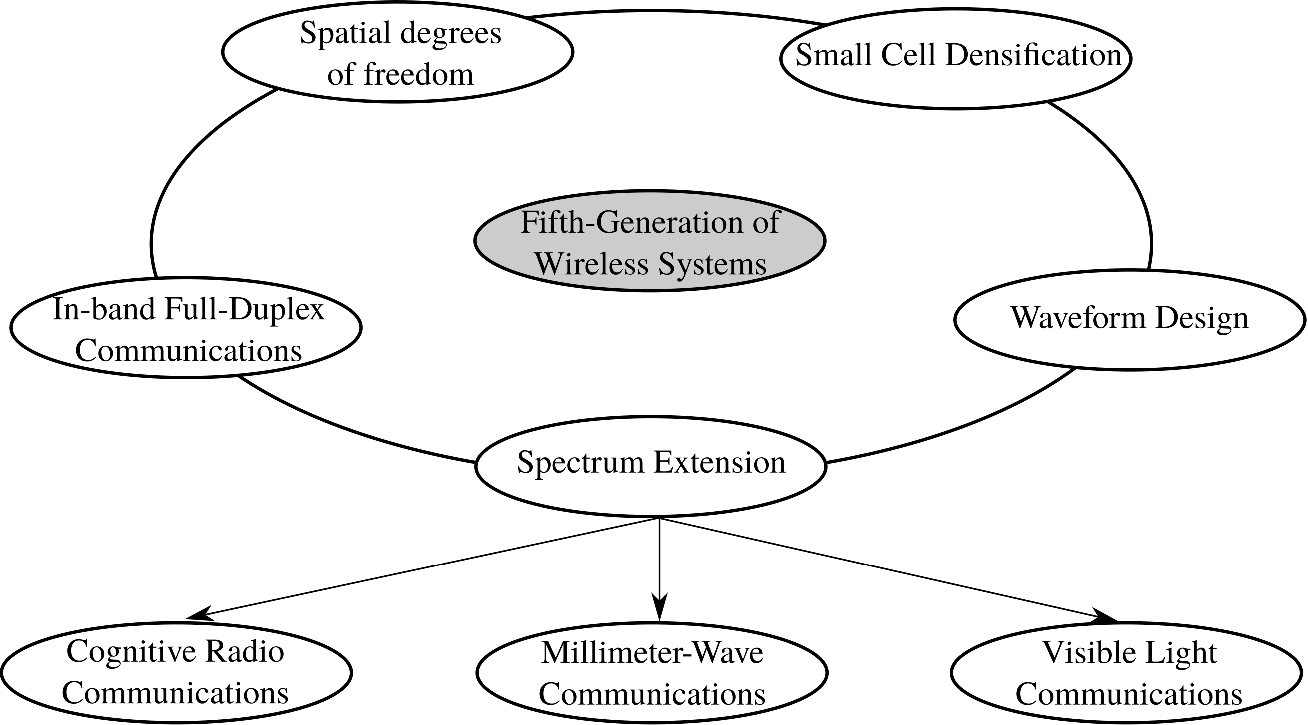
\includegraphics[width = 0.75\columnwidth]{figures/5G.ps}
        	};	
		%\node[draw = none,align=center] (A) at (0.23,0.53) {> \SI{6}{GHz}};
		\only<1>
		{
		\draw[decorate, decoration={brace, amplitude=10pt}, xshift = -4pt, yshift=0pt] (0.0,-0.7) -- (2.8,-0.7) node[black,midway,yshift=+0.5cm] {< \SI{6}{GHz}};
		\draw[decorate, decoration={brace, amplitude=10pt}, xshift = -4pt, yshift=0pt] (3.15,-0.7) -- (5.95,-0.7) node[black,midway,yshift=+0.5cm] {\SI{6}{GHz} -- \SI{300}{GHz}};
		\draw[decorate, decoration={brace, amplitude=10pt}, xshift = -4pt, yshift=0pt] (6.3,-0.7) -- (9.1,-0.7) node[black,midway,yshift=+0.5cm] {\SI{430}{THz} -- \SI{770}{THz}};
		%\draw[-latex] (B) edge (A);
		}
		\only<1-2>
		{
			\fill[opacity = 0.4, fill = kit-green30] (-0.1,-0.4) rectangle (8.9,2.2);
		}
		\only<3->
		{
			\draw[opacity = 0, decorate, decoration={brace, amplitude=10pt}, xshift = -4pt, yshift=0pt] (0.0,-0.7) -- (2.8,-0.7) node[black,midway,yshift=+0.5cm] {< \SI{6}{GHz}};
			\draw[opacity = 0, decorate, decoration={brace, amplitude=10pt}, xshift = -4pt, yshift=0pt] (3.15,-0.7) -- (5.95,-0.7) node[black,midway,yshift=+0.5cm] {\SI{6}{GHz} -- \SI{300}{GHz}};
			\draw[opacity = 0, decorate, decoration={brace, amplitude=10pt}, xshift = -4pt, yshift=0pt] (6.3,-0.7) -- (9.1,-0.7) node[black,midway,yshift=+0.5cm] {\SI{430}{THz} -- \SI{770}{THz}};
			\fill[opacity = 0.4, fill = kit-green30] (-0.1,-0.4) rectangle (2.7,1.15);
		}
		\end{tikzpicture}
	\end{center}
	\end{overlayarea}
	\begin{center}
		\only<1>
		{
			\tikzfancyarrow[11.0cm][kit-green70][top color=kit-green30, bottom color=kit-green50, shape border rotate=0]{Electromagnetic Spectrum}
		}
		\only<2>
		{
			\tikzfancyarrow[11.0cm][kit-green70][top color=kit-green30, bottom color=kit-green50, shape border rotate=180]{Mobility}
		}
		\only<3>
		{
			\begin{block}{}
			A Cognitive Radio (CR) is an agile system that allows efficient usage (secondary access) of the spectrum below $\SI{6}{Hz}$ 
			\end{block}
		}
	\end{center}
\end{frame}


%%%%%%%%%%%%%%%%%%%%%%%%%%%%%%%%%%%%%%%%%%%%%%%%%%%%%%%%%%%%%%%%%%%%%%%%%%%%%%%%
\begin{frame}[t]{Cognitive Small Cell}
%%%%%%%%%%%%%%%%%%%%%%%%%%%%%%%%%%%%%%%%%%%%%%%%%%%%%%%%%%%%%%%%%%%%%%%%%%%%%%%%
		\vspace{-0.3cm}
		\fs{7}{8}
		\begin{block}{}%{\scriptsize Cognitive Small Cell?}
		An Cognitive Small Cell (CSC) is a network entity that enable CR communications for the devices operating indoor 
		\end{block}
	\begin{columns}
	\begin{column}{0.37\columnwidth}
		\vspace{-0.1cm}
		\only<1,3->
		{	
			\begin{block}{\scriptsize Network Elements}
				\begin{itemize}
					\item Cognitive Small Cell-Base Station ($\color{blue}{\text{CSC-BS}}$)
					\item Mobile Station ($\color{green}{\text{MS}}$) 
					\item Macro Cell-Base Station ($\color{red}{\text{MC-BS}}$) 
				\end{itemize}
			\end{block}
		}
		\only<2>
		{
			\begin{block}{\scriptsize \textbf{Network Elements}}
				\begin{itemize}
					\item Cognitive Small Cell-Base Station ($\color{blue}{\text{CSC-BS}}$)
					\item Mobile Station ($\color{green}{\text{MS}}$) 
					\item Macro Cell-Base Station ($\color{red}{\text{MC-BS}}$) 
				\end{itemize}
			\end{block}
		}
		\only<1,2,4->
		{
			\begin{block}{\scriptsize Spectrum Access}
				\begin{itemize}
					\item Wireless backhaul link ($\color{blue}{\text{CSC-BS} \Leftrightarrow \text{MC-BS}}$)
					\item Direct link ($\color{green}{\text{MC-BS} \Leftrightarrow \text{MS}}$) 
					\item Indirect link ($\color{red}{\text{CSC-BS} \Leftrightarrow \text{MS}}$) 
				\end{itemize}
			\end{block}
		}
		\only<3>
		{
			\begin{block}{\scriptsize \textbf{Spectrum Access}}
				\begin{itemize}
					\item Wireless backhaul link ($\color{blue}{\text{CSC-BS} \Leftrightarrow \text{MC-BS}}$)
					\item Direct link ($\color{green}{\text{MC-BS} \Leftrightarrow \text{MS}}$) 
					\item Indirect link ($\color{red}{\text{CSC-BS} \Leftrightarrow \text{MS}}$) 
				\end{itemize}
			\end{block}
		}
		\only<1-3>
		{
			\begin{block}{\scriptsize Indoor?}
				\begin{itemize}
					\item 70\% traffic is originated indoor $\Leftrightarrow$ Traffic Management
					\item Spatial separation $\Leftrightarrow$ Interference suppression	
				\end{itemize}
			\end{block}
		}
		\only<4->
		{
			\begin{block}{\scriptsize \textbf{Indoor?}}
				\begin{itemize}
					\item 70\% traffic is originated indoor $\Leftrightarrow$ Traffic Management
					\item Spatial separation $\Leftrightarrow$ Interference suppression	
				\end{itemize}
			\end{block}
		}
	\end{column}
	\begin{column}{0.63\columnwidth}
		\fs{7}{8}
		\begin{center}
			CSC in a preliminary 5G network \\\vspace{0.4cm} 
        		\begin{tikzpicture}[scale=1]
				\node[anchor=south west,inner sep=0] (image) at (0,0)
				{
					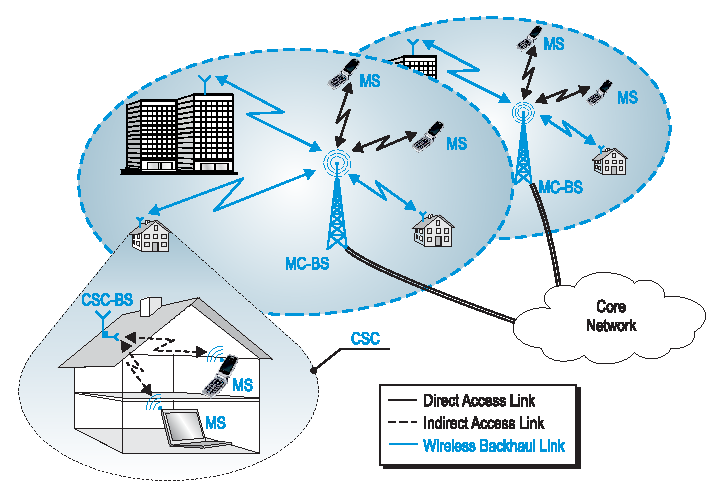
\includegraphics[width = \columnwidth]{../kapitel01/figures/Cellular_Scenario_CR6F}	     
				};
				\only<2>
				{
					\fill[opacity = 0.2, fill = blue] (0.65,1.47) rectangle (1.28,2.03);
					\fill[opacity = 0.2, fill = green] (1.5,.33) rectangle (2.32,.81);
					\fill[opacity = 0.2, fill = red] (2.8,2.2) rectangle (3.59,3.57);
				}
				\only<3>
				{
					\fill[opacity = 0.2, fill = blue] (1.37,2.78) rectangle (3.2,3.35);
					\fill[opacity = 0.2, fill = green] (3.35,3.5) rectangle (3.6,4.3);
					\fill[opacity = 0.2, fill = red] (1.08,0.89) rectangle (2.05,1.61);
				}
			\end{tikzpicture}	
		\end{center}
	\end{column}
	\end{columns}
\end{frame}

\subsection{Performance Analysis}
%%%%%%%%%%%%%%%%%%%%%%%%%%%%%%%%%%%%%%%%%%%%%%%%%%%%%%%%%%%%%%%%%%%%%%%%%%%%%%%%
\begin{frame}[t]{Performance Analysis of CR System}
%%%%%%%%%%%%%%%%%%%%%%%%%%%%%%%%%%%%%%%%%%%%%%%%%%%%%%%%%%%%%%%%%%%%%%%%%%%%%%%%
	% Performance analysis us determine the hardware feasibility of a wireless system. In context to CR system it is a critical.  
	\vspace{-3mm}
	\fs{7}{8}
	\begin{block}{\scriptsize Challenges}
		\begin{itemize}
			% Complexity of the underlying scenario. Coexistence illustrates sharing a chunk of spectrum. Different with respect to the wireless technologies and in terms of privilege for the access 
			\item Involves the coexistence of two different system: {\color{blue}{primary}} and {\color{red}{secondary}} 
			% For system design one assume no knowledge about the primary user signal 
			\item With no concrete guidelines available in the literature $\Leftrightarrow$ no knowledge about the primary user signal is a reasonable assumption
			% With regard to the above issues 
			\item Existing theoretical analysis rarely converges to an hardware implementation $\Leftrightarrow$ deployment perspective % in order words, rarely deal(tackle) the problem from a deployment perspective 
		\end{itemize}
	\end{block}
	\vspace{-1mm}
	\begin{columns}
		\begin{column}{0.37\columnwidth}
			\onslide<2->
			{
				\begin{block}{\scriptsize Performance characterization}
					Upon applying CR techniques at ST, a CR system grantees\begin{itemize}
						\item Protection to primary system $\Leftrightarrow$ interference power at PR 
						\item QoE to secondary system $\Leftrightarrow$ at SR 
					\end{itemize}
				\end{block}
			}
			\vspace{-1mm}
			\onslide<3->
			{
				\begin{block}{}%{\scriptsize Channel knowledge}
					Knowledge of interacting channels is absolutely necessary at ST 
				\end{block}
			}
			\onslide<4->
	 		{
				\centering
				\tikzfancyarrow[0.85cm][kit-green70][top color=kit-green50, bottom color=kit-green50, shape border rotate=270]{\color{kit-green50}{10}}			\\[0.5em]	
	               		\begin{tikzpicture}[scale=1]
	               	 		\node[draw=none,fill=gray!30, minimum height = 0.5cm, align = center] at (0.0, 0.0) {Channel Estimation is proposed at ST/SR};
				\end{tikzpicture}
			}
		\end{column}
		\begin{column}{0.63\columnwidth}
		\vspace{-1mm}
		\fs{7}{8}
		\begin{center}
			% Interacting entities
			{\color{blue}{PT, PR}}, \color{red}{ST($\Leftrightarrow$ CSC-BS) and SR($\Leftrightarrow$ MS)}\\\vspace{0.2cm} 
        		\begin{tikzpicture}[scale=1]
				\node[anchor=south west,inner sep=0] (image) at (0,0)
				{
					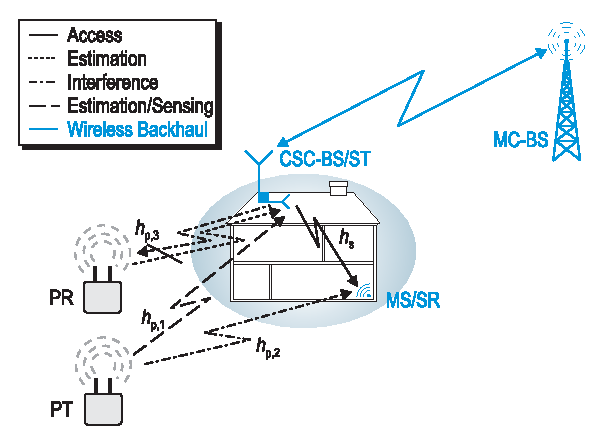
\includegraphics[width = 0.85\columnwidth]{../kapitel01/figures/CR_Scenario_Hybrid}	     
				};
				\only<1>
				{
					\fill[opacity = 0.2, fill = blue] (.32,1.16) rectangle (1.22,1.8);
					\fill[opacity = 0.2, fill = blue] (.32,-0.06) rectangle (1.22,0.58);
					\fill[opacity = 0.2, fill = red] (3.65,1.18) rectangle (4.65,1.6);
					\fill[opacity = 0.2, fill = red] (2.42,2.3) rectangle (3.88,3.08);
				}
				\only<2>
				{
					\draw[blue, thick] (.32,1.16) rectangle (1.22,1.8); %PR
					\draw[red, thick] (3.65,1.18) rectangle (4.65,1.6); %ST
					\draw[red, thick] (2.42,2.3) rectangle (3.88,3.08); %SR
					
					%% Dummy figure added to avoid a shift between two slides
					\fill[opacity = 0.0, fill = blue] (.32,-0.06) rectangle (1.22,0.58);
				}
				\only<3->
				{
					
					\fill[opacity = 0.2, fill = gray!70] (1.28,.98) rectangle (1.68,1.34);
					\fill[opacity = 0.2, fill = gray!70] (1.22,1.96) rectangle (1.62,2.32);
					\fill[opacity = 0.2, fill = gray!70] (3.38,1.86) rectangle (3.78,2.22);
					\fill[opacity = 0.2, fill = gray!70] (2.52,.68) rectangle (2.92,1.04);
					
					%% Dummy figure added to avoid a shift between two slides
					\fill[opacity = 0.0, fill = blue] (.32,-0.06) rectangle (1.22,0.58);
				}
				\only<4->
				{
					\draw[red, thick] (3.65,1.18) rectangle (4.65,1.6); %ST
					\draw[red, thick] (2.42,2.3) rectangle (3.88,3.08); %SR
				}
			\end{tikzpicture}	
		\end{center}
		\end{column}
	\end{columns}
\end{frame}


%%%%%%%%%%%%%%%%%%%%%%%%%%%%%%%%%%%%%%%%%%%%%%%%%%%%%%%%%%%%%%%%%%%%%%%%%%%%%%%%
\begin{frame}[t]{Major Contributions}
%%%%%%%%%%%%%%%%%%%%%%%%%%%%%%%%%%%%%%%%%%%%%%%%%%%%%%%%%%%%%%%%%%%%%%%%%%%%%%%%
	\vspace{-1.5mm}
	\begin{columns}
		\begin{column}[t]{0.53\columnwidth}
			\centering Challenges: \\[-0.2em]
				\fs{7}{8}
				% Choice of the estimation technique
				\begin{block}{\scriptsize Estimation Technique?} %{\scriptsize Challenges}
					Estimation of channels between two different systems %$\Rightarrow$ 
					\begin{itemize}
					% There exits a multitude of wireless standards that can act as primary system, it is difficult to included a dedicated circuitry for each primary user signal 
						\item Complexity and versatility towards unknown primary user signals
						\item Conventional techniques are not feasible  
					\end{itemize}
				\end{block}
				\vspace{-1.1mm}
				\onslide<2->
				{
				\begin{block}{\scriptsize System Design aspects?} %of incorporating channel estimation on the performance
					\begin{itemize} 
						\item How to tackle the variations induced? 
						\item Time allocation for channel estimation 
						%\item Channel fading 
					\end{itemize}
				\end{block}
				}
				\vspace{-1.1mm}
				\onslide<3->
				{
				\begin{block}{\scriptsize Impact on performance?}%{\scriptsize Channel knowledge}
					\begin{itemize}
						\item Primary system's performance? $\Rightarrow$ interference 
						\item Secondary system's performance? $\Rightarrow$ throughput 
					\end{itemize} 
				\end{block}
				}	
				\vspace{-1.1mm}
				\onslide<4->
				{
				\begin{block}{\scriptsize Hardware Feasibility?}%{\scriptsize Channel knowledge}
					\begin{itemize}
					\item Validity of the assumptions made? 
					\item Applicability of the proposed framework under realistic scenarios? 
					\end{itemize}	
				\end{block}
				}
		\end{column}
		
		\begin{column}{0.03\columnwidth}
		\end{column}
		
		\begin{column}[t]{0.44\columnwidth}
			\centering Proposed Solutions: \\[-0.2em]
				\fs{7}{8}
			\fs{7}{8}
			\begin{block}{}
				\centering
				Received power based channel estimation
				%\begin{itemize}
					%\item 
					Low-complexity and versatility requirements are satisfied  
					%\item Incorporation of received power in performance characterization 
				%\end{itemize}
			\end{block}
			\vspace{-0.5mm}
			\onslide<2->
			{
			\begin{block}{}
				\centering
			  	Stochastic modeling \\ To characterize the variations 	
			\end{block}
			\vspace{-0.5mm}
			\begin{block}{}
				\centering
			   	Time allocation for channel estimation in secondary user's frame structure
			\end{block}
			}
			\vspace{-0.5mm}
			\onslide<3->
			{
			\begin{block}{}
				\centering
			  	Interference constraints  \\To protect PR from harmful interference 
			\end{block}
			}	
			\vspace{-0.5mm}
			\onslide<3->
			{
			\begin{block}{}
				\centering
			 	Performance tradeoffs \\ To determine suitable estimation time that determines the achievable throughput	
			\end{block}
			}
			\vspace{-0.4mm}
			\onslide<4->
			{
			\begin{block}{}%{\scriptsize Hardware Feasibility}%{\scriptsize Channel knowledge}			
				\centering
				Empirical validation \\ Hardware demonstration
				%\begin{itemize}
					%\item Empirical validation %of the derived expressions
					%\item Hardware demonstration %of a CR system
				%\end{itemize}	
			\end{block}
			}
		\end{column}
	\end{columns}
\end{frame}

%%%%%%%%%%%%%%%%%%%%%%%%%%%%%%%%%%%%%%%%%%%%%%%%%%%%%%%%%%%%%%%%%%%%%%%%%%%%%%%%%
%\begin{frame}[c]{Contributions}
%%%%%%%%%%%%%%%%%%%%%%%%%%%%%%%%%%%%%%%%%%%%%%%%%%%%%%%%%%%%%%%%%%%%%%%%%%%%%%%%%
%	\vspace{-2mm}
%	%\hspace{-2mm}
%	\begin{center}
%	\begin{tikzpicture}[scale=1]
%                                \node[anchor=south west,inner sep=0] (image) at (0,0)
%                                {
%                                        \includegraphics[width = 1.0\columnwidth]{../kapitel01/figures/Contri.ps}
%                                };
%                        \end{tikzpicture}
%	\end{center}
%\end{frame}

\fi

\ifinter
\section{Interweave System}
%%%%%%%%%%%%%%%%%%%%%%%%%%%%%%%%%%%%%%%%%%%%%%%%%%%%%%%%%%%%%%%%%%%%%%%%%%%%%%%%
\begin{frame}[c]{}
%%%%%%%%%%%%%%%%%%%%%%%%%%%%%%%%%%%%%%%%%%%%%%%%%%%%%%%%%%%%%%%%%%%%%%%%%%%%%%%%
\begin{center}
Interweave System
\end{center}
\end{frame}

%%%%%%%%%%%%%%%%%%%%%%%%%%%%%%%%%%%%%%%%%%%%%%%%%%%%%%%%%%%%%%%%%%%%%%%%%%%%%%%%
\begin{frame}[t]{Interweave System}
%%%%%%%%%%%%%%%%%%%%%%%%%%%%%%%%%%%%%%%%%%%%%%%%%%%%%%%%%%%%%%%%%%%%%%%%%%%%%%%%
	\vspace{-2mm}
	\fs{7}{8}
	\begin{columns}
		\begin{column}{0.44\columnwidth}
				%\vspace{-1mm}
			\begin{block}{\scriptsize Principle} %{\scriptsize Principle}
				\begin{itemize}
					\item Interweave system employs spectrum sensing at the ST 
					\item Spectrum sensing is CR technique used for detecting the signals transmitted by PT
					%\item Energy detector is employed 
				\end{itemize}
			\end{block}
			\vspace{-1mm}
			\onslide<2->
			{
				\begin{block}{\scriptsize Signal model} %{\scriptsize Signal model}
				\begin{equation*}
					\yrcvd[n] = 
					\begin{cases}
					\hpo \cdot \xp[n] + \wst[n] & : \mathcal{H}_1 \\
					\wst[n] & :\mathcal{H}_0
					\end{cases}
					%\label{eq_IS:sys_mod_p1s}
				\end{equation*}
				\begin{equation*}
					\ys[n] = 
					\begin{cases}
						\hs \cdot \xs[n] + \hpt \cdot \xp[n] +  \wsr[n] & \\%: 1 - \pd \\
						\hs \cdot \xs[n] + \wsr[n] & %: 1 - \pfa
					\end{cases}
					\label{eq_IS:sys_mod_ss}
				\end{equation*}
				\end{block}
				\vspace{-1mm}
				\begin{block}{\scriptsize Energy detector's performance} %Detector performance Interference at PR is dependent on the detectors performance
				\begin{equation*}
						\pd = \Gamma\left( \frac{\tsen \fsam}{2}, \frac{\tsen \fsam \mu}{2 \color{red}{\prcvdstpt}} \right), %\\ 
				\end{equation*}	
				\begin{equation*}
						\pfa = \Gamma\left( \frac{\tsen \fsam}{2}, \frac{\tsen \fsam \mu}{2 \npo} \right)%,  \label{eq_IS:pfa} 
				\end{equation*}	
				\end{block}	
			}
		\end{column}
		\begin{column}{0.56\columnwidth}
		\vspace{6mm}
		\fs{7}{8}
		\begin{center}
			% Interacting entities
			%Interweave Scenario \\\vspace{0.2cm} 
        		\begin{tikzpicture}[scale=1]
				\node[anchor=south west,inner sep=0] (image) at (0,0)
				{
					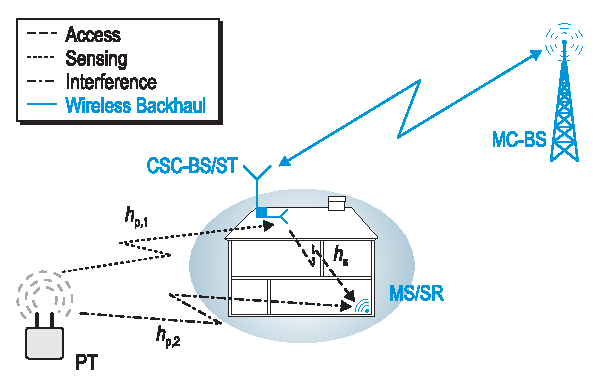
\includegraphics[width = 0.9\columnwidth]{../kapitel03/figures/CR_Scenario_Interweave}	     
				};
				\only<1>
				{
					%\fill[opacity = 0.2, fill = blue] (.32,1.16) rectangle (1.22,1.8);
					%\fill[opacity = 0.2, fill = blue] (.32,-0.06) rectangle (1.22,0.58);
					%\fill[opacity = 0.2, fill = red] (3.65,1.18) rectangle (4.65,1.6);
					%\fill[opacity = 0.2, fill = red] (2.42,2.3) rectangle (3.88,3.08);
				}
			\end{tikzpicture}	
		\end{center}
		\begin{block}{\scriptsize Secondary throughput} %Secondary throughput
                                \vspace{-2.6mm}
				\begin{align*}
                               		\rs(\tsen) =& \frac{T- \tsen}{T} \bigg[ \log_2 \left(1 + {\color{red}{|\hs|^2}} \frac{\ptranst}{\npo}\right) (1 - \pfa) \phz  \\ & + \log_2 \left(1 + \frac{{\color{red}{|\hs|^2}} \ptranst }{{\color{red}{|\hpt|^2}} \ptranpt  + \npo } \right)  (1 - \pd) \pho  \bigg] 
				\end{align*} 
                \end{block} 
		\end{column}
	\end{columns}
\end{frame}

%%%%%%%%%%%%%%%%%%%%%%%%%%%%%%%%%%%%%%%%%%%%%%%%%%%%%%%%%%%%%%%%%%%%%%%%%%%%%%%%
\begin{frame}[t]{Interweave System}
%%%%%%%%%%%%%%%%%%%%%%%%%%%%%%%%%%%%%%%%%%%%%%%%%%%%%%%%%%%%%%%%%%%%%%%%%%%%%%%%
	\vspace{-2mm}
	\fs{7}{8}
	%\begin{block}{}
	%\end{block}			
	\begin{columns}
		\begin{column}{0.38\columnwidth}
			%\vspace{-1mm}
			\begin{block}{\scriptsize Ideal Model (IM)}
     			   	\vspace{-4.5mm}
	    		        \begin{align*}
				\trs(\ttsen) &= \maxi_{\tsen} \trs(\tsen)\\ 
				\text{s.t.} & \text{ } \pd \ge \pdd	
	        	\end{align*}
			%Without the knowledge of channel gains $\phpo$, $\phpt$ and $\phs$, it is difficult to characterize the performance parameters $\pd$ and $\rs$  
			\end{block}
			\vspace{-1.5mm}
			\begin{block}{\scriptsize Proposed Approach}
			\begin{center}
			\begin{tikzpicture}[node distance = 1.27cm, auto]
                        	% draw nodes
				\node [block] (frame) {Incorporation of time resources for channel estimation and sensing in frame structure ($\test, \tsen$)};
  			        \node [block, below of=frame] (channelest) {Variations ($\epgpo$, $\epgpt$, $\epgs$) due to channel estimation are characterized in terms of $\fpgpo, \fpgpt, \fpgs$};
  			        \node [block, below of=channelest] (cdf) {Variations in performance parameters ($\epd$, $\ecz$, $\eco$) are characterized in terms of $\fpd, \fcz, \fco$};
  			        \node [block, below of=cdf] (tradeoff) {The cdfs are used to determine the achievable secondary throughput subject to interference constraints};
				% draw edges
    				\path [line] (frame) -- (channelest);
    				\path [line] (channelest) -- (cdf);
    				\path [line] (cdf) -- (tradeoff);
			\end{tikzpicture}
			\end{center}
			\end{block}

		\end{column}
		\begin{column}{0.62\columnwidth}
		\fs{7}{8}
		\begin{center}
        		%Frame Structure \\\vspace{2mm}
			\begin{overlayarea}{\textwidth}{4.1cm}
			\begin{tikzpicture}[scale=1]
				\node[anchor=south west,inner sep=0] (image) at (0,0)
				{
					\includegraphics[width = \columnwidth]{figures/Frame_Structure_IS.ps}     
				};
			\end{tikzpicture}	
                        \end{overlayarea}
			\vspace{3.5mm}
			\begin{overlayarea}{\textwidth}{2.6cm}
			\only<1>
			{	
				\begin{block}{\scriptsize Estimation Model (EM) -- Average Constraint (AC)} 
                               	 \vspace{-3.2mm}
					\begin{align*}
					\trsac(\ttest, \ttsenac) =& \maxi_{\test, \tsen} \e{\epd, \ecz, \eco}{\rs(\test, \tsen)},	\\	
					\text{s.t.} & \text{ }  \e{\epd}{\epd} \ge \pdd, \\ 
\text{s.t.} & \text{ }  0 < \test \le \tsen \le T
					\end{align*} 
               		 	\end{block}
			} 
			\only<2->
			{	
				\begin{block}{\scriptsize Estimation Model (EM) -- Outage Constraint (OC)} 
                               	 \vspace{-3.2mm}
					\begin{align*}
					\trsac(\ttest, \ttsenac) =& \maxi_{\test, \tsen} \e{\epd, \ecz, \eco}{\rs(\test, \tsen)},	\\	
					\text{s.t.} & \text{ }  \p(\epd \le \pdd) \le \mpd, \\
\text{s.t.} & \text{ }  0 < \test \le \tsen \le T
					\end{align*} 
               		 	\end{block}
			} 
                        \end{overlayarea}
		\end{center}
		\end{column}
	\end{columns}
\end{frame}


%%%%%%%%%%%%%%%%%%%%%%%%%%%%%%%%%%%%%%%%%%%%%%%%%%%%%%%%%%%%%%%%%%%%%%%%%%%%%%%%
\begin{frame}[t]{Interweave System}
%%%%%%%%%%%%%%%%%%%%%%%%%%%%%%%%%%%%%%%%%%%%%%%%%%%%%%%%%%%%%%%%%%%%%%%%%%%%%%%%
	\vspace{-2mm}
	\begin{columns}
	\begin{column}{0.45\columnwidth}
	\fs{7}{8}
		\renewcommand{\arraystretch}{1.55}
		\begin{tabular}{c||c}
		%\hline
		\rowcolor{kit-green30}
		Parameter & Value \\
		\hline\hline
		$\fsam$ & $\SI{1}{MHz}$ \\ %\hline
		$\phpo$ & $\SI{-100}{dB}$ \\ %\hline
		$\phpt$ & $\SI{-100}{dB}$ \\ %\hline
		$\phs$ & $\SI{-80}{dB}$ \\ %\hline 
		$T$ & $\SI{100}{ms}$ \\ %\hline 
		$\npo$ & $\SI{-100}{dBm}$ \\ %\hline
		$\snrrcvd$ & $\SI{-10}{dB}$ \\ %\hline
		$\snrpt$ & $\SI{-10}{dB}$ \\ %\hline
		$\snrso$ & $\SI{10}{dB}$ \\ %\hline
		%$\ptranpt$ & $-\SI{10}{dBm}$ \\ %\hline
		%$\ptranst$ & $-\SI{10}{dBm}$ \\ %\hline
		$\pho = 1 - \phz$ & 0.2 \\ %\hline
		%$\test$ & $\SI{5}{ms}$ \\ %\hline
		$\Ks$ & 10 \\ \hline
		%$\Kp$ & $1000$ \\ \hline
	\end{tabular}

	\end{column}
	\begin{column}{0.55\columnwidth}
	\begin{center}
	\fs{7}{8}	
		%% Add psfrag entries
		% This file is generated by the MATLAB m-file laprint.m. It can be included
% into LaTeX documents using the packages graphicx, color and psfrag.
% It is accompanied by a postscript file. A sample LaTeX file is:
%    \documentclass{article}\usepackage{graphicx,color,psfrag}
%    \begin{document}% This file is generated by the MATLAB m-file laprint.m. It can be included
% into LaTeX documents using the packages graphicx, color and psfrag.
% It is accompanied by a postscript file. A sample LaTeX file is:
%    \documentclass{article}\usepackage{graphicx,color,psfrag}
%    \begin{document}% This file is generated by the MATLAB m-file laprint.m. It can be included
% into LaTeX documents using the packages graphicx, color and psfrag.
% It is accompanied by a postscript file. A sample LaTeX file is:
%    \documentclass{article}\usepackage{graphicx,color,psfrag}
%    \begin{document}\input{fig_opt_thr_vs_est_time_diff_mu_AWGN}\end{document}
% See http://www.mathworks.de/matlabcentral/fileexchange/loadFile.do?objectId=4638
% for recent versions of laprint.m.
%
% created by:           LaPrint version 3.16 (13.9.2004)
% created on:           12-Jul-2016 15:03:36
% eps bounding box:     16 cm x 12 cm
% comment:              
%
%\begin{psfrags}%
%\psfragscanon%
%
% text strings:
\psfrag{s05}[b][b]{\fontsize{8}{12}\fontseries{m}\mathversion{normal}\fontshape{n}\selectfont \color[rgb]{0,0,0}\setlength{\tabcolsep}{0pt}\begin{tabular}{c}$\trs(\test,\ttsen)$ [bits/sec/Hz]\end{tabular}}%
\psfrag{s06}[t][t]{\fontsize{8}{12}\fontseries{m}\mathversion{normal}\fontshape{n}\selectfont \color[rgb]{0,0,0}\setlength{\tabcolsep}{0pt}\begin{tabular}{c}$\test$ [ms]\end{tabular}}%
\psfrag{s10}[][]{\fontsize{10}{15}\fontseries{m}\mathversion{normal}\fontshape{n}\selectfont \color[rgb]{0,0,0}\setlength{\tabcolsep}{0pt}\begin{tabular}{c} \end{tabular}}%
\psfrag{s11}[][]{\fontsize{10}{15}\fontseries{m}\mathversion{normal}\fontshape{n}\selectfont \color[rgb]{0,0,0}\setlength{\tabcolsep}{0pt}\begin{tabular}{c} \end{tabular}}%
\psfrag{s12}[l][l]{\fontsize{8}{12}\fontseries{m}\mathversion{normal}\fontshape{n}\selectfont \color[rgb]{0,0,0}$\trs(\ttest,\ttsen)$}%
\psfrag{s13}[l][l]{\fontsize{8}{12}\fontseries{m}\mathversion{normal}\fontshape{n}\selectfont \color[rgb]{0,0,0}IM}%
\psfrag{s14}[l][l]{\fontsize{8}{12}\fontseries{m}\mathversion{normal}\fontshape{n}\selectfont \color[rgb]{0,0,0}EM-AC, Problem 1}%
\psfrag{s15}[l][l]{\fontsize{8}{12}\fontseries{m}\mathversion{normal}\fontshape{n}\selectfont \color[rgb]{0,0,0}EM-OC, Problem 2}%
\psfrag{s16}[l][l]{\fontsize{8}{12}\fontseries{m}\mathversion{normal}\fontshape{n}\selectfont \color[rgb]{0,0,0}Corollary 1}%
\psfrag{s17}[l][l]{\fontsize{8}{12}\fontseries{m}\mathversion{normal}\fontshape{n}\selectfont \color[rgb]{0,0,0}$\trs(\ttest,\ttsen)$}%
%
% axes font properties:
\fontsize{8}{12}\fontseries{m}\mathversion{normal}%
\fontshape{n}\selectfont%
%
% xticklabels:
\psfrag{x01}[t][t]{1}%
\psfrag{x02}[t][t]{2}%
\psfrag{x03}[t][t]{3}%
\psfrag{x04}[t][t]{4}%
\psfrag{x05}[t][t]{5}%
\psfrag{x06}[t][t]{6}%
\psfrag{x07}[t][t]{7}%
\psfrag{x08}[t][t]{8}%
\psfrag{x09}[t][t]{9}%
\psfrag{x10}[t][t]{10}%
%
% yticklabels:
\psfrag{v01}[r][r]{1.8}%
\psfrag{v02}[r][r]{1.9}%
\psfrag{v03}[r][r]{2}%
\psfrag{v04}[r][r]{2.1}%
\psfrag{v05}[r][r]{2.2}%
\psfrag{v06}[r][r]{2.3}%
\psfrag{v07}[r][r]{2.4}%
\psfrag{v08}[r][r]{2.5}%
\psfrag{v09}[r][r]{2.6}%
\psfrag{v10}[r][r]{2.7}%
%
% Figure:
%\resizebox{8cm}{!}{\includegraphics{fig_opt_thr_vs_est_time_diff_mu_AWGN.eps}}%
%\end{psfrags}%
%
% End fig_opt_thr_vs_est_time_diff_mu_AWGN.tex
\end{document}
% See http://www.mathworks.de/matlabcentral/fileexchange/loadFile.do?objectId=4638
% for recent versions of laprint.m.
%
% created by:           LaPrint version 3.16 (13.9.2004)
% created on:           12-Jul-2016 15:03:36
% eps bounding box:     16 cm x 12 cm
% comment:              
%
%\begin{psfrags}%
%\psfragscanon%
%
% text strings:
\psfrag{s05}[b][b]{\fontsize{8}{12}\fontseries{m}\mathversion{normal}\fontshape{n}\selectfont \color[rgb]{0,0,0}\setlength{\tabcolsep}{0pt}\begin{tabular}{c}$\trs(\test,\ttsen)$ [bits/sec/Hz]\end{tabular}}%
\psfrag{s06}[t][t]{\fontsize{8}{12}\fontseries{m}\mathversion{normal}\fontshape{n}\selectfont \color[rgb]{0,0,0}\setlength{\tabcolsep}{0pt}\begin{tabular}{c}$\test$ [ms]\end{tabular}}%
\psfrag{s10}[][]{\fontsize{10}{15}\fontseries{m}\mathversion{normal}\fontshape{n}\selectfont \color[rgb]{0,0,0}\setlength{\tabcolsep}{0pt}\begin{tabular}{c} \end{tabular}}%
\psfrag{s11}[][]{\fontsize{10}{15}\fontseries{m}\mathversion{normal}\fontshape{n}\selectfont \color[rgb]{0,0,0}\setlength{\tabcolsep}{0pt}\begin{tabular}{c} \end{tabular}}%
\psfrag{s12}[l][l]{\fontsize{8}{12}\fontseries{m}\mathversion{normal}\fontshape{n}\selectfont \color[rgb]{0,0,0}$\trs(\ttest,\ttsen)$}%
\psfrag{s13}[l][l]{\fontsize{8}{12}\fontseries{m}\mathversion{normal}\fontshape{n}\selectfont \color[rgb]{0,0,0}IM}%
\psfrag{s14}[l][l]{\fontsize{8}{12}\fontseries{m}\mathversion{normal}\fontshape{n}\selectfont \color[rgb]{0,0,0}EM-AC, Problem 1}%
\psfrag{s15}[l][l]{\fontsize{8}{12}\fontseries{m}\mathversion{normal}\fontshape{n}\selectfont \color[rgb]{0,0,0}EM-OC, Problem 2}%
\psfrag{s16}[l][l]{\fontsize{8}{12}\fontseries{m}\mathversion{normal}\fontshape{n}\selectfont \color[rgb]{0,0,0}Corollary 1}%
\psfrag{s17}[l][l]{\fontsize{8}{12}\fontseries{m}\mathversion{normal}\fontshape{n}\selectfont \color[rgb]{0,0,0}$\trs(\ttest,\ttsen)$}%
%
% axes font properties:
\fontsize{8}{12}\fontseries{m}\mathversion{normal}%
\fontshape{n}\selectfont%
%
% xticklabels:
\psfrag{x01}[t][t]{1}%
\psfrag{x02}[t][t]{2}%
\psfrag{x03}[t][t]{3}%
\psfrag{x04}[t][t]{4}%
\psfrag{x05}[t][t]{5}%
\psfrag{x06}[t][t]{6}%
\psfrag{x07}[t][t]{7}%
\psfrag{x08}[t][t]{8}%
\psfrag{x09}[t][t]{9}%
\psfrag{x10}[t][t]{10}%
%
% yticklabels:
\psfrag{v01}[r][r]{1.8}%
\psfrag{v02}[r][r]{1.9}%
\psfrag{v03}[r][r]{2}%
\psfrag{v04}[r][r]{2.1}%
\psfrag{v05}[r][r]{2.2}%
\psfrag{v06}[r][r]{2.3}%
\psfrag{v07}[r][r]{2.4}%
\psfrag{v08}[r][r]{2.5}%
\psfrag{v09}[r][r]{2.6}%
\psfrag{v10}[r][r]{2.7}%
%
% Figure:
%\resizebox{8cm}{!}{\includegraphics{fig_opt_thr_vs_est_time_diff_mu_AWGN.eps}}%
%\end{psfrags}%
%
% End fig_opt_thr_vs_est_time_diff_mu_AWGN.tex
\end{document}
% See http://www.mathworks.de/matlabcentral/fileexchange/loadFile.do?objectId=4638
% for recent versions of laprint.m.
%
% created by:           LaPrint version 3.16 (13.9.2004)
% created on:           12-Jul-2016 15:03:36
% eps bounding box:     16 cm x 12 cm
% comment:              
%
%\begin{psfrags}%
%\psfragscanon%
%
% text strings:
\psfrag{s05}[b][b]{\fontsize{8}{12}\fontseries{m}\mathversion{normal}\fontshape{n}\selectfont \color[rgb]{0,0,0}\setlength{\tabcolsep}{0pt}\begin{tabular}{c}$\trs(\test,\ttsen)$ [bits/sec/Hz]\end{tabular}}%
\psfrag{s06}[t][t]{\fontsize{8}{12}\fontseries{m}\mathversion{normal}\fontshape{n}\selectfont \color[rgb]{0,0,0}\setlength{\tabcolsep}{0pt}\begin{tabular}{c}$\test$ [ms]\end{tabular}}%
\psfrag{s10}[][]{\fontsize{10}{15}\fontseries{m}\mathversion{normal}\fontshape{n}\selectfont \color[rgb]{0,0,0}\setlength{\tabcolsep}{0pt}\begin{tabular}{c} \end{tabular}}%
\psfrag{s11}[][]{\fontsize{10}{15}\fontseries{m}\mathversion{normal}\fontshape{n}\selectfont \color[rgb]{0,0,0}\setlength{\tabcolsep}{0pt}\begin{tabular}{c} \end{tabular}}%
\psfrag{s12}[l][l]{\fontsize{8}{12}\fontseries{m}\mathversion{normal}\fontshape{n}\selectfont \color[rgb]{0,0,0}$\trs(\ttest,\ttsen)$}%
\psfrag{s13}[l][l]{\fontsize{8}{12}\fontseries{m}\mathversion{normal}\fontshape{n}\selectfont \color[rgb]{0,0,0}IM}%
\psfrag{s14}[l][l]{\fontsize{8}{12}\fontseries{m}\mathversion{normal}\fontshape{n}\selectfont \color[rgb]{0,0,0}EM-AC, Problem 1}%
\psfrag{s15}[l][l]{\fontsize{8}{12}\fontseries{m}\mathversion{normal}\fontshape{n}\selectfont \color[rgb]{0,0,0}EM-OC, Problem 2}%
\psfrag{s16}[l][l]{\fontsize{8}{12}\fontseries{m}\mathversion{normal}\fontshape{n}\selectfont \color[rgb]{0,0,0}Corollary 1}%
\psfrag{s17}[l][l]{\fontsize{8}{12}\fontseries{m}\mathversion{normal}\fontshape{n}\selectfont \color[rgb]{0,0,0}$\trs(\ttest,\ttsen)$}%
%
% axes font properties:
\fontsize{8}{12}\fontseries{m}\mathversion{normal}%
\fontshape{n}\selectfont%
%
% xticklabels:
\psfrag{x01}[t][t]{1}%
\psfrag{x02}[t][t]{2}%
\psfrag{x03}[t][t]{3}%
\psfrag{x04}[t][t]{4}%
\psfrag{x05}[t][t]{5}%
\psfrag{x06}[t][t]{6}%
\psfrag{x07}[t][t]{7}%
\psfrag{x08}[t][t]{8}%
\psfrag{x09}[t][t]{9}%
\psfrag{x10}[t][t]{10}%
%
% yticklabels:
\psfrag{v01}[r][r]{1.8}%
\psfrag{v02}[r][r]{1.9}%
\psfrag{v03}[r][r]{2}%
\psfrag{v04}[r][r]{2.1}%
\psfrag{v05}[r][r]{2.2}%
\psfrag{v06}[r][r]{2.3}%
\psfrag{v07}[r][r]{2.4}%
\psfrag{v08}[r][r]{2.5}%
\psfrag{v09}[r][r]{2.6}%
\psfrag{v10}[r][r]{2.7}%
%
% Figure:
%\resizebox{8cm}{!}{\includegraphics{fig_opt_thr_vs_est_time_diff_mu_AWGN.eps}}%
%\end{psfrags}%
%
% End fig_opt_thr_vs_est_time_diff_mu_AWGN.tex

		\centering
                \resizebox{.95 \columnwidth}{!}{%
			\begin{tikzpicture}[scale=1]
			\node[anchor=south west,inner sep=0] (image) at (0,0)
			{
				\includegraphics[width= 1.2\columnwidth]{../kapitel03/figures/fig_opt_thr_vs_est_time_diff_mu_AWGN}
			};
			\begin{scope}[x={(image.south east)},y={(image.north west)}]
			\draw[black,->, thick] (0.25,0.64) -- (0.18,0.84);
			\node[draw=none, font=\scriptsize] at (0.35, 0.58) {$\mpd \in \{0.05,0.10,0.15\}$};

			\draw[black,<-, thick] (0.75,0.62) -- (0.75,0.915);
			\node[draw=none, font=\scriptsize] at (0.75,0.58) {Performance degradation}; 
			%\draw[black,->] (0.25,0.6) node[below =12.0,right=-20.0,  font=\scriptsize] {$\mpd \in \{0.05,0.10,0.15\}$} -- (0.18,0.8);

			%\draw[help lines,xstep=.1,ystep=.1] (0,0) grid (1,1);
			%\foreach \x in {0,1,...,9} { \node [anchor=north] at (\x/10,0) {0.\x}; }
			%\foreach \y in {0,1,...,9} { \node [anchor=east] at (0,\y/10) {0.\y}; }
	               	\node[draw=none,fill=kit-green30, minimum height = 0.6cm, align = center, font = \footnotesize] at (0.5, 1.05) {Secondary throughput versus estimation time};
			\end{scope}
			\end{tikzpicture}
		}
	\end{center}
	\end{column}
	\end{columns}
	\begin{block}{}
		\fs{7}{8}
		\begin{itemize}
			\item Ideal model is used as a benchmark $\Rightarrow$ evaluate degradation in performance due to inclusion of channel estimation
			%\item Outage constraint is a severe interference constraint in comparison to average constraint 

			\item Tradeoff between the estimation time and the secondary throughput 
		\end{itemize}		
	\end{block}	
\end{frame}

\fi

\section{Underlay System}
%%%%%%%%%%%%%%%%%%%%%%%%%%%%%%%%%%%%%%%%%%%%%%%%%%%%%%%%%%%%%%%%%%%%%%%%%%%%%%%%
\begin{frame}[c]{}
%%%%%%%%%%%%%%%%%%%%%%%%%%%%%%%%%%%%%%%%%%%%%%%%%%%%%%%%%%%%%%%%%%%%%%%%%%%%%%%%
\begin{center}
Underlay System
\end{center}
\end{frame}

%%%%%%%%%%%%%%%%%%%%%%%%%%%%%%%%%%%%%%%%%%%%%%%%%%%%%%%%%%%%%%%%%%%%%%%%%%%%%%%%
\begin{frame}[t]{Underlay System}
%%%%%%%%%%%%%%%%%%%%%%%%%%%%%%%%%%%%%%%%%%%%%%%%%%%%%%%%%%%%%%%%%%%%%%%%%%%%%%%%
	\vspace{-4mm}
	\fs{7}{8}
	\begin{columns}
		\begin{column}{0.44\columnwidth}
				%\vspace{-1mm}
			\begin{block}{\scriptsize Principle} %{\scriptsize Principle}
				\begin{itemize}
					%\item Underlay systems correspond to a interference tolerant systems
					\item Power control mechanism is employed at ST 
					\item ST listens to control signal transmitted by PR 
					%\item Spectrum sensing is CR technique used for detecting the signals transmitted by PT
					%\item Energy detector is employed 
				\end{itemize}
			\end{block}
			\vspace{2mm}
			\onslide<1->
			{
				\begin{block}{\scriptsize Signal model} %{\scriptsize Signal model}
				\begin{equation*}
					\yrcvd[n] = \hpth \cdot \xtran[n] + \wsr[n]
				\end{equation*}
				\begin{equation*}
					\yp[n] = \hpth  \cdot \xreg[n] + \wpr[n]
				\end{equation*}
				\begin{equation*}
					\ys[n] = \gs \cdot \xreg[n] + \gpt \cdot \xp[n] + \wsr[n]
				\end{equation*}
				\end{block}
				\vspace{2mm}
				\begin{block}{\scriptsize Ideal Model} 
				%Interference received at PR\\[-.2em]	
				\begin{equation*}
					\prcvdpr = \phpth \preg \le \ite
				\end{equation*}	
				%Data rate at SR\\[-.2em]	
				\begin{equation*}
					\ca = \log_2 \left(1 + \frac{\pgs \preg}{ \pgpt \ptranpt + \nps} \right)	
				\end{equation*}	
				\end{block}	
			}
		\end{column}
		\begin{column}{0.56\columnwidth}
		\vspace{-6mm}
		\fs{7}{8}
		\begin{center}
			% Interacting entities
			%Interweave Scenario \\\vspace{0.2cm} 
        		\begin{tikzpicture}[scale=1]
				\node[anchor=south west,inner sep=0] (image) at (0,0)
				{
					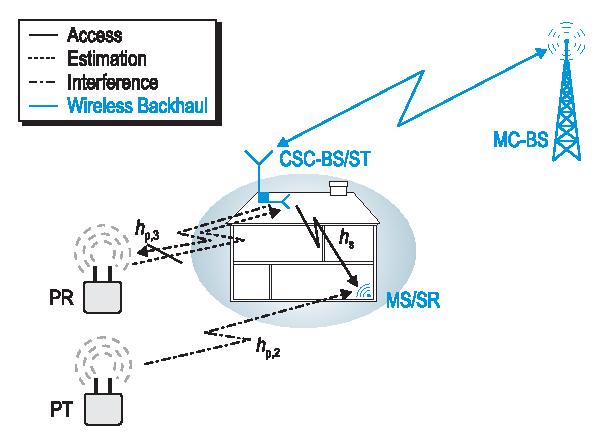
\includegraphics[width = .81 \columnwidth]{../kapitel04/figures/CR_Scenario_Underlay}	     
				};
				\only<1>
				{
					%\fill[opacity = 0.2, fill = blue] (.32,1.16) rectangle (1.22,1.8);
					%\fill[opacity = 0.2, fill = blue] (.32,-0.06) rectangle (1.22,0.58);
					%\fill[opacity = 0.2, fill = red] (3.65,1.18) rectangle (4.65,1.6);
					%\fill[opacity = 0.2, fill = red] (2.42,2.3) rectangle (3.88,3.08);
				}
			\end{tikzpicture}
			\vspace{-10mm}	
			\begin{tikzpicture}[scale=1]
				\node[anchor=south west,inner sep=0] (image) at (0,0)
				{
					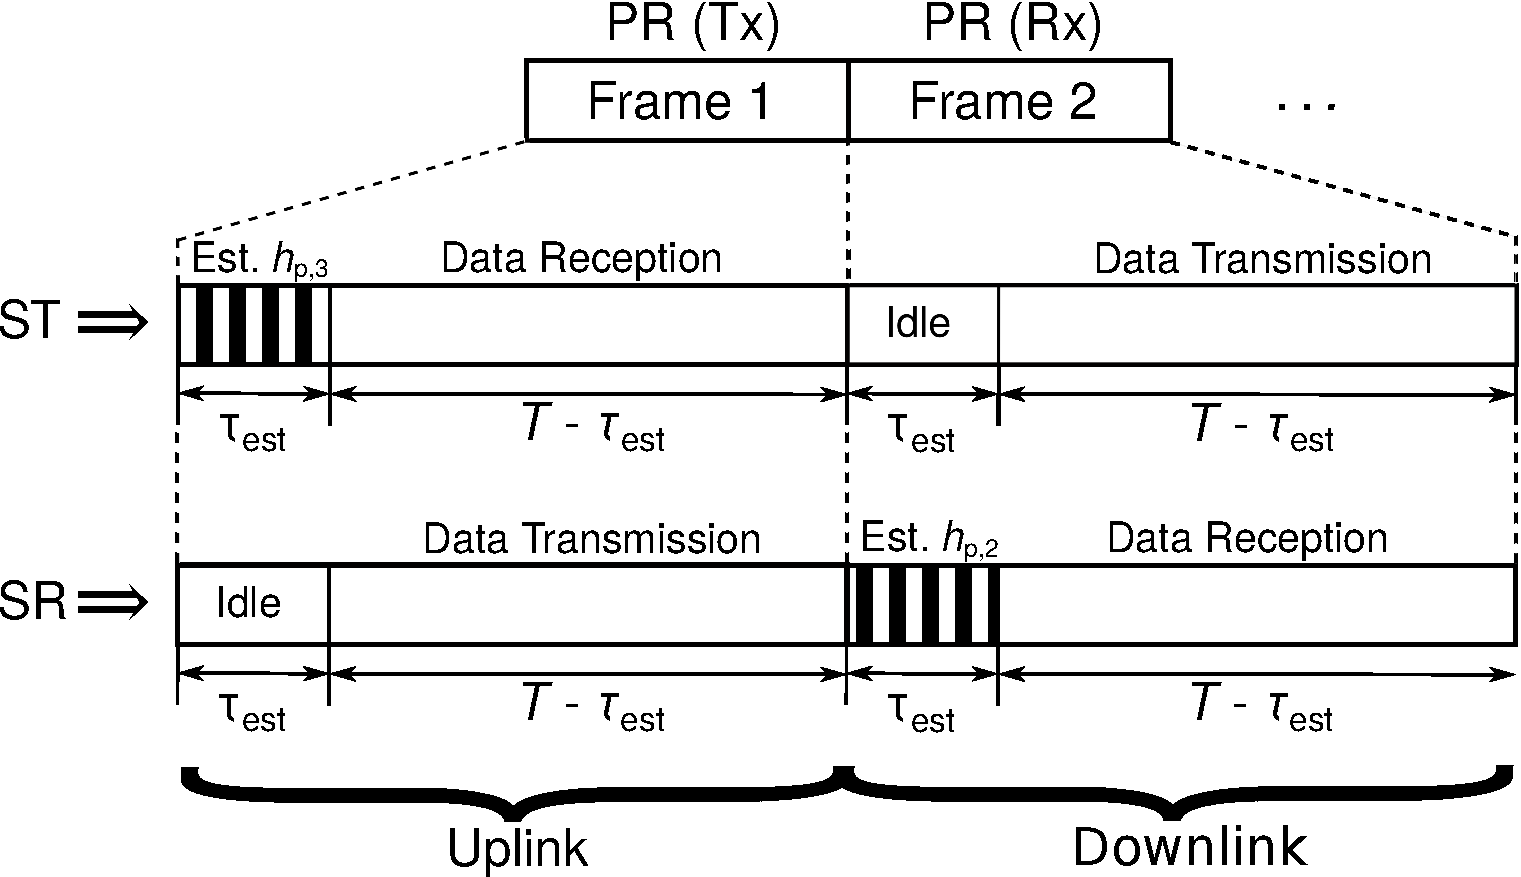
\includegraphics[width = \columnwidth]{figures/Frame_Structure_US.ps}     
				};
			\end{tikzpicture}	
		\end{center}
		\end{column}
	\end{columns}
\end{frame}


%%%%%%%%%%%%%%%%%%%%%%%%%%%%%%%%%%%%%%%%%%%%%%%%%%%%%%%%%%%%%%%%%%%%%%%%%%%%%%%%
\begin{frame}[t]{Underlay System}
%%%%%%%%%%%%%%%%%%%%%%%%%%%%%%%%%%%%%%%%%%%%%%%%%%%%%%%%%%%%%%%%%%%%%%%%%%%%%%%%
	\vspace{-4.5mm}
	\fs{7}{8}
	\begin{columns}
		\begin{column}{0.45\columnwidth}
			\begin{block}{\scriptsize Control Power} %{\scriptsize Principle}
			Constraint on received interference at PR 
			\begin{align*}
				\p\left( \prcvdpr = \ephpth \preg \ge \ite \right) \le \opc, \\  
				\p\left( \left( \frac{\eprcvdstpr - \nps}{\ptran}\right) \preg \ge \ite \right) \le \opc 
			\end{align*}
			Constraint on transmit power at ST 
			\begin{equation*}
				\preg \le \pc. \label{eq_US:pc} 
			\end{equation*}
			\end{block} 
			\vspace{-3mm}
			\begin{center}	
				\tikzfancyarrow[0.9cm][kit-green70][top color=kit-green50, bottom color=kit-green50, shape border rotate=270]{\color{kit-green50}{10}}		%	\\[0.5em]
			\end{center}	
		\end{column}
		\begin{column}{0.55\columnwidth}
		\fs{7}{8}
		\begin{center}
			%% Add psfrag entries
                	% This file is generated by the MATLAB m-file laprint.m. It can be included
% into LaTeX documents using the packages graphicx, color and psfrag.
% It is accompanied by a postscript file. A sample LaTeX file is:
%    \documentclass{article}\usepackage{graphicx,color,psfrag}
%    \begin{document}% This file is generated by the MATLAB m-file laprint.m. It can be included
% into LaTeX documents using the packages graphicx, color and psfrag.
% It is accompanied by a postscript file. A sample LaTeX file is:
%    \documentclass{article}\usepackage{graphicx,color,psfrag}
%    \begin{document}% This file is generated by the MATLAB m-file laprint.m. It can be included
% into LaTeX documents using the packages graphicx, color and psfrag.
% It is accompanied by a postscript file. A sample LaTeX file is:
%    \documentclass{article}\usepackage{graphicx,color,psfrag}
%    \begin{document}\input{fig_Preg_est_time_AWGN}\end{document}
% See http://www.mathworks.de/matlabcentral/fileexchange/loadFile.do?objectId=4638
% for recent versions of laprint.m.
%
% created by:           LaPrint version 3.16 (13.9.2004)
% created on:           15-Dec-2015 22:25:07
% eps bounding box:     16 cm x 12 cm
% comment:              
%
%\begin{psfrags}%
%\psfragscanon%
%
% text strings:
\psfrag{s05}[b][b]{\fontsize{8.5}{12.75}\fontseries{m}\mathversion{normal}\fontshape{n}\selectfont \color[rgb]{0,0,0}\setlength{\tabcolsep}{0pt}\begin{tabular}{c}$\preg$ [dBm]\end{tabular}}%
\psfrag{s06}[t][t]{\fontsize{8.5}{12.75}\fontseries{m}\mathversion{normal}\fontshape{n}\selectfont \color[rgb]{0,0,0}\setlength{\tabcolsep}{0pt}\begin{tabular}{c}$\test$ [ms]\end{tabular}}%
\psfrag{s10}[][]{\fontsize{10}{15}\fontseries{m}\mathversion{normal}\fontshape{n}\selectfont \color[rgb]{0,0,0}\setlength{\tabcolsep}{0pt}\begin{tabular}{c} \end{tabular}}%
\psfrag{s11}[][]{\fontsize{10}{15}\fontseries{m}\mathversion{normal}\fontshape{n}\selectfont \color[rgb]{0,0,0}\setlength{\tabcolsep}{0pt}\begin{tabular}{c} \end{tabular}}%
\psfrag{s12}[l][l]{\fontsize{8.5}{12.75}\fontseries{m}\mathversion{normal}\fontshape{n}\selectfont \color[rgb]{0,0,0}EM}%
\psfrag{s13}[l][l]{\fontsize{8.5}{12.75}\fontseries{m}\mathversion{normal}\fontshape{n}\selectfont \color[rgb]{0,0,0}IM}%
\psfrag{s14}[l][l]{\fontsize{8.5}{12.75}\fontseries{m}\mathversion{normal}\fontshape{n}\selectfont \color[rgb]{0,0,0}EM}%
%
% axes font properties:
\fontsize{8.5}{12.75}\fontseries{m}\mathversion{normal}%
\fontshape{n}\selectfont%
%
% xticklabels:
\psfrag{x01}[t][t]{$10^{-3}$}%
\psfrag{x02}[t][t]{$10^{-2}$}%
\psfrag{x03}[t][t]{$10^{-1}$}%
\psfrag{x04}[t][t]{$10^{0}$}%
\psfrag{x05}[t][t]{$10^{1}$}%
%
% yticklabels:
\psfrag{v01}[r][r]{-20}%
\psfrag{v02}[r][r]{-19}%
\psfrag{v03}[r][r]{-18}%
\psfrag{v04}[r][r]{-17}%
\psfrag{v05}[r][r]{-16}%
\psfrag{v06}[r][r]{-15}%
\psfrag{v07}[r][r]{-14}%
\psfrag{v08}[r][r]{-13}%
\psfrag{v09}[r][r]{-12}%
\psfrag{v10}[r][r]{-11}%
\psfrag{v11}[r][r]{-10}%
\psfrag{v12}[r][r]{-9}%
%
% Figure:
%\resizebox{8cm}{!}{\includegraphics{fig_Preg_est_time_AWGN.eps}}%
%\end{psfrags}%
%
% End fig_Preg_est_time_AWGN.tex
\end{document}
% See http://www.mathworks.de/matlabcentral/fileexchange/loadFile.do?objectId=4638
% for recent versions of laprint.m.
%
% created by:           LaPrint version 3.16 (13.9.2004)
% created on:           15-Dec-2015 22:25:07
% eps bounding box:     16 cm x 12 cm
% comment:              
%
%\begin{psfrags}%
%\psfragscanon%
%
% text strings:
\psfrag{s05}[b][b]{\fontsize{8.5}{12.75}\fontseries{m}\mathversion{normal}\fontshape{n}\selectfont \color[rgb]{0,0,0}\setlength{\tabcolsep}{0pt}\begin{tabular}{c}$\preg$ [dBm]\end{tabular}}%
\psfrag{s06}[t][t]{\fontsize{8.5}{12.75}\fontseries{m}\mathversion{normal}\fontshape{n}\selectfont \color[rgb]{0,0,0}\setlength{\tabcolsep}{0pt}\begin{tabular}{c}$\test$ [ms]\end{tabular}}%
\psfrag{s10}[][]{\fontsize{10}{15}\fontseries{m}\mathversion{normal}\fontshape{n}\selectfont \color[rgb]{0,0,0}\setlength{\tabcolsep}{0pt}\begin{tabular}{c} \end{tabular}}%
\psfrag{s11}[][]{\fontsize{10}{15}\fontseries{m}\mathversion{normal}\fontshape{n}\selectfont \color[rgb]{0,0,0}\setlength{\tabcolsep}{0pt}\begin{tabular}{c} \end{tabular}}%
\psfrag{s12}[l][l]{\fontsize{8.5}{12.75}\fontseries{m}\mathversion{normal}\fontshape{n}\selectfont \color[rgb]{0,0,0}EM}%
\psfrag{s13}[l][l]{\fontsize{8.5}{12.75}\fontseries{m}\mathversion{normal}\fontshape{n}\selectfont \color[rgb]{0,0,0}IM}%
\psfrag{s14}[l][l]{\fontsize{8.5}{12.75}\fontseries{m}\mathversion{normal}\fontshape{n}\selectfont \color[rgb]{0,0,0}EM}%
%
% axes font properties:
\fontsize{8.5}{12.75}\fontseries{m}\mathversion{normal}%
\fontshape{n}\selectfont%
%
% xticklabels:
\psfrag{x01}[t][t]{$10^{-3}$}%
\psfrag{x02}[t][t]{$10^{-2}$}%
\psfrag{x03}[t][t]{$10^{-1}$}%
\psfrag{x04}[t][t]{$10^{0}$}%
\psfrag{x05}[t][t]{$10^{1}$}%
%
% yticklabels:
\psfrag{v01}[r][r]{-20}%
\psfrag{v02}[r][r]{-19}%
\psfrag{v03}[r][r]{-18}%
\psfrag{v04}[r][r]{-17}%
\psfrag{v05}[r][r]{-16}%
\psfrag{v06}[r][r]{-15}%
\psfrag{v07}[r][r]{-14}%
\psfrag{v08}[r][r]{-13}%
\psfrag{v09}[r][r]{-12}%
\psfrag{v10}[r][r]{-11}%
\psfrag{v11}[r][r]{-10}%
\psfrag{v12}[r][r]{-9}%
%
% Figure:
%\resizebox{8cm}{!}{\includegraphics{fig_Preg_est_time_AWGN.eps}}%
%\end{psfrags}%
%
% End fig_Preg_est_time_AWGN.tex
\end{document}
% See http://www.mathworks.de/matlabcentral/fileexchange/loadFile.do?objectId=4638
% for recent versions of laprint.m.
%
% created by:           LaPrint version 3.16 (13.9.2004)
% created on:           15-Dec-2015 22:25:07
% eps bounding box:     16 cm x 12 cm
% comment:              
%
%\begin{psfrags}%
%\psfragscanon%
%
% text strings:
\psfrag{s05}[b][b]{\fontsize{8.5}{12.75}\fontseries{m}\mathversion{normal}\fontshape{n}\selectfont \color[rgb]{0,0,0}\setlength{\tabcolsep}{0pt}\begin{tabular}{c}$\preg$ [dBm]\end{tabular}}%
\psfrag{s06}[t][t]{\fontsize{8.5}{12.75}\fontseries{m}\mathversion{normal}\fontshape{n}\selectfont \color[rgb]{0,0,0}\setlength{\tabcolsep}{0pt}\begin{tabular}{c}$\test$ [ms]\end{tabular}}%
\psfrag{s10}[][]{\fontsize{10}{15}\fontseries{m}\mathversion{normal}\fontshape{n}\selectfont \color[rgb]{0,0,0}\setlength{\tabcolsep}{0pt}\begin{tabular}{c} \end{tabular}}%
\psfrag{s11}[][]{\fontsize{10}{15}\fontseries{m}\mathversion{normal}\fontshape{n}\selectfont \color[rgb]{0,0,0}\setlength{\tabcolsep}{0pt}\begin{tabular}{c} \end{tabular}}%
\psfrag{s12}[l][l]{\fontsize{8.5}{12.75}\fontseries{m}\mathversion{normal}\fontshape{n}\selectfont \color[rgb]{0,0,0}EM}%
\psfrag{s13}[l][l]{\fontsize{8.5}{12.75}\fontseries{m}\mathversion{normal}\fontshape{n}\selectfont \color[rgb]{0,0,0}IM}%
\psfrag{s14}[l][l]{\fontsize{8.5}{12.75}\fontseries{m}\mathversion{normal}\fontshape{n}\selectfont \color[rgb]{0,0,0}EM}%
%
% axes font properties:
\fontsize{8.5}{12.75}\fontseries{m}\mathversion{normal}%
\fontshape{n}\selectfont%
%
% xticklabels:
\psfrag{x01}[t][t]{$10^{-3}$}%
\psfrag{x02}[t][t]{$10^{-2}$}%
\psfrag{x03}[t][t]{$10^{-1}$}%
\psfrag{x04}[t][t]{$10^{0}$}%
\psfrag{x05}[t][t]{$10^{1}$}%
%
% yticklabels:
\psfrag{v01}[r][r]{-20}%
\psfrag{v02}[r][r]{-19}%
\psfrag{v03}[r][r]{-18}%
\psfrag{v04}[r][r]{-17}%
\psfrag{v05}[r][r]{-16}%
\psfrag{v06}[r][r]{-15}%
\psfrag{v07}[r][r]{-14}%
\psfrag{v08}[r][r]{-13}%
\psfrag{v09}[r][r]{-12}%
\psfrag{v10}[r][r]{-11}%
\psfrag{v11}[r][r]{-10}%
\psfrag{v12}[r][r]{-9}%
%
% Figure:
%\resizebox{8cm}{!}{\includegraphics{fig_Preg_est_time_AWGN.eps}}%
%\end{psfrags}%
%
% End fig_Preg_est_time_AWGN.tex

			\centering
             	        \resizebox{.95 \columnwidth}{!}{%
                        \begin{tikzpicture}[scale=1]
				\node[anchor=south west,inner sep=0] (image) at (0,0)
				{
					\includegraphics[width= 1.2\columnwidth]{../kapitel04/figures/fig_Preg_est_time_AWGN}
				};
				\begin{scope}[x={(image.south east)},y={(image.north west)}]

				\draw (0.35,0.56) arc(-130:130:0.007 and 0.021);
				\node[draw,fill=gray!10,font=\scriptsize] at (0.44,0.515) {$\opc = 0.01$};

				\draw (0.35,0.68) arc(-130:130:0.007 and 0.021);
				\node[draw,fill=gray!10,font=\scriptsize] at (0.275,0.758) {$\opc = 0.1$};

	               		\node[draw=none,fill=kit-green30, minimum height = 0.6cm, align = center, font = \footnotesize] at (0.5, 1.05) {Controlled power versus estimation time};
				%\draw[help lines,xstep=.1,ystep=.1] (0,0) grid (1,1);
				%\foreach \x in {0,1,...,9} { \node [anchor=north] at (\x/10,0) {0.\x}; }
				%\foreach \y in {0,1,...,9} { \node [anchor=east] at (0,\y/10) {0.\y}; }
				\end{scope}
			\end{tikzpicture}
                }
		\end{center}
		\end{column}
	\end{columns}
	\begin{block}{}%{\scriptsize Power control} 
		\vspace{-4mm}
		\begin{align*}
			\preg &= 
			\begin{cases} 
				\frac{\ite \ptran}{ \left(\bpo \Gamma^{-1}(\opc, \apo) - \nps  \right)}, & \mbox{for } \preg < \pc \\
				\pc, & \mbox{for } \preg \ge \pc
				\end{cases} \\
				\text{where  } \apo &= \frac{\test \fsam (1 + \snrrcvdu)^2}{2 + 4 \snrrcvdu} \text{ and } \bpo = \frac{\nps (2 + 4 \snrrcvdu)}{\test \fsam (1 + \snrrcvdu)},
			\end{align*}
	\end{block}
\end{frame}


%%%%%%%%%%%%%%%%%%%%%%%%%%%%%%%%%%%%%%%%%%%%%%%%%%%%%%%%%%%%%%%%%%%%%%%%%%%%%%%%
\begin{frame}[t]{Underlay System}
%%%%%%%%%%%%%%%%%%%%%%%%%%%%%%%%%%%%%%%%%%%%%%%%%%%%%%%%%%%%%%%%%%%%%%%%%%%%%%%%
	\vspace{-4.5mm}
	\fs{7}{8}
	\begin{columns}
		\begin{column}{0.45\columnwidth}
			\begin{block}{\scriptsize Secondary throughput} %{\scriptsize Principle}
			\vspace{-3mm}
			\begin{align*}
				\eca  = \log_2 \left(1 + \frac{\epgs \preg}{\eprcvdsr} \right) \\
				\rs(\test) = \frac{T - \test}{T} \e{\eca} {\eca} 
			\end{align*}
			\end{block}

			\begin{block}{\scriptsize Achievable secondary throughput} 
			\vspace{-3mm}
			\begin{align*}
				\trs(\ttest)  = \maxi_{\test}  & \text{      } {\rs(\test)} \\
				\text{s.t.} & \;\p\left( \ephpth \preg \ge \ite \right) \le \opc \\
				\text{s.t.} & \;\preg \le \pc
			\end{align*}
			\end{block}
		\end{column}
		\begin{column}{0.55\columnwidth}
		\fs{7}{8}
		\begin{center}
			%% Add psfrag entries
                	% This file is generated by the MATLAB m-file laprint.m. It can be included
% into LaTeX documents using the packages graphicx, color and psfrag.
% It is accompanied by a postscript file. A sample LaTeX file is:
%    \documentclass{article}\usepackage{graphicx,color,psfrag}
%    \begin{document}% This file is generated by the MATLAB m-file laprint.m. It can be included
% into LaTeX documents using the packages graphicx, color and psfrag.
% It is accompanied by a postscript file. A sample LaTeX file is:
%    \documentclass{article}\usepackage{graphicx,color,psfrag}
%    \begin{document}% This file is generated by the MATLAB m-file laprint.m. It can be included
% into LaTeX documents using the packages graphicx, color and psfrag.
% It is accompanied by a postscript file. A sample LaTeX file is:
%    \documentclass{article}\usepackage{graphicx,color,psfrag}
%    \begin{document}\input{fig_thr_est_time_tradeoff_AWGN}\end{document}
% See http://www.mathworks.de/matlabcentral/fileexchange/loadFile.do?objectId=4638
% for recent versions of laprint.m.
%
% created by:           LaPrint version 3.16 (13.9.2004)
% created on:           08-Jan-2016 12:22:27
% eps bounding box:     16 cm x 12 cm
% comment:              
%
%\begin{psfrags}%
%\psfragscanon%
%
% text strings:
\psfrag{s05}[b][b]{\fontsize{8.5}{12.75}\fontseries{m}\mathversion{normal}\fontshape{n}\selectfont \color[rgb]{0,0,0}\setlength{\tabcolsep}{0pt}\begin{tabular}{c}$\rs(\tau)$ [bits/sec/Hz]\end{tabular}}%
\psfrag{s06}[t][t]{\fontsize{8.5}{12.75}\fontseries{m}\mathversion{normal}\fontshape{n}\selectfont \color[rgb]{0,0,0}\setlength{\tabcolsep}{0pt}\begin{tabular}{c}$\tau$ [ms]\end{tabular}}%
\psfrag{s10}[][]{\fontsize{10}{15}\fontseries{m}\mathversion{normal}\fontshape{n}\selectfont \color[rgb]{0,0,0}\setlength{\tabcolsep}{0pt}\begin{tabular}{c} \end{tabular}}%
\psfrag{s11}[][]{\fontsize{10}{15}\fontseries{m}\mathversion{normal}\fontshape{n}\selectfont \color[rgb]{0,0,0}\setlength{\tabcolsep}{0pt}\begin{tabular}{c} \end{tabular}}%
\psfrag{s12}[l][l]{\fontsize{8.5}{12.75}\fontseries{m}\mathversion{normal}\fontshape{n}\selectfont \color[rgb]{0,0,0}Simulated}%
\psfrag{s13}[l][l]{\fontsize{8.5}{12.75}\fontseries{m}\mathversion{normal}\fontshape{n}\selectfont \color[rgb]{0,0,0}IM}%
\psfrag{s14}[l][l]{\fontsize{8.5}{12.75}\fontseries{m}\mathversion{normal}\fontshape{n}\selectfont \color[rgb]{0,0,0}EM}%
\psfrag{s15}[l][l]{\fontsize{8.5}{12.75}\fontseries{m}\mathversion{normal}\fontshape{n}\selectfont \color[rgb]{0,0,0}$\trs(\ttau)$}%
\psfrag{s16}[l][l]{\fontsize{8.5}{12.75}\fontseries{m}\mathversion{normal}\fontshape{n}\selectfont \color[rgb]{0,0,0}Simulated}%
%
% axes font properties:
\fontsize{8.5}{12.75}\fontseries{m}\mathversion{normal}%
\fontshape{n}\selectfont%
%
% xticklabels:
\psfrag{x01}[t][t]{0}%
\psfrag{x02}[t][t]{1}%
\psfrag{x03}[t][t]{2}%
\psfrag{x04}[t][t]{3}%
\psfrag{x05}[t][t]{4}%
\psfrag{x06}[t][t]{5}%
\psfrag{x07}[t][t]{6}%
\psfrag{x08}[t][t]{7}%
\psfrag{x09}[t][t]{8}%
\psfrag{x10}[t][t]{9}%
\psfrag{x11}[t][t]{10}%
%
% yticklabels:
\psfrag{v01}[r][r]{1.6}%
\psfrag{v02}[r][r]{1.8}%
\psfrag{v03}[r][r]{2}%
\psfrag{v04}[r][r]{2.2}%
\psfrag{v05}[r][r]{2.4}%
\psfrag{v06}[r][r]{2.6}%
%
% Figure:
%\resizebox{8cm}{!}{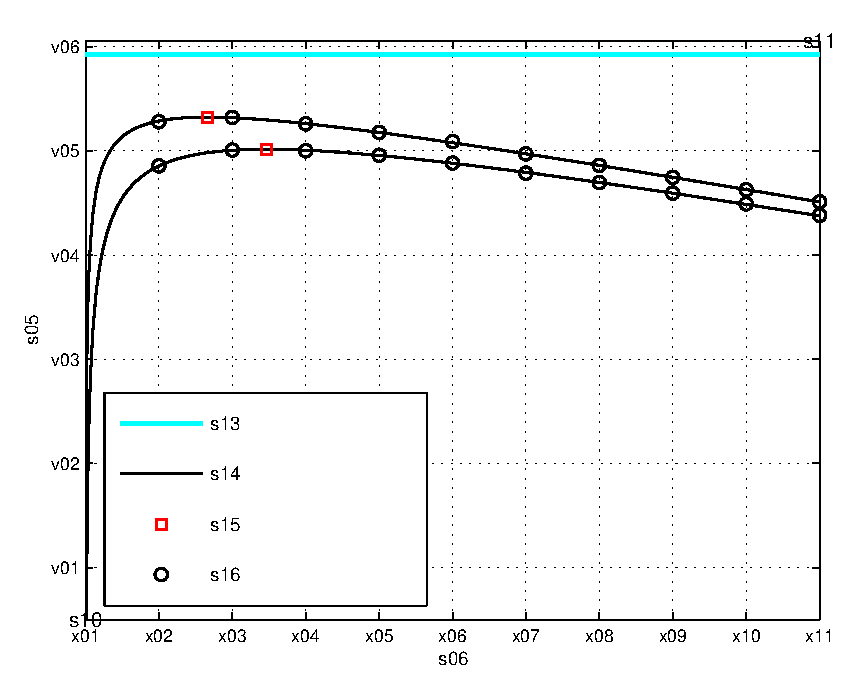
\includegraphics{fig_thr_est_time_tradeoff_AWGN.eps}}%
%\end{psfrags}%
%
% End fig_thr_est_time_tradeoff_AWGN.tex
\end{document}
% See http://www.mathworks.de/matlabcentral/fileexchange/loadFile.do?objectId=4638
% for recent versions of laprint.m.
%
% created by:           LaPrint version 3.16 (13.9.2004)
% created on:           08-Jan-2016 12:22:27
% eps bounding box:     16 cm x 12 cm
% comment:              
%
%\begin{psfrags}%
%\psfragscanon%
%
% text strings:
\psfrag{s05}[b][b]{\fontsize{8.5}{12.75}\fontseries{m}\mathversion{normal}\fontshape{n}\selectfont \color[rgb]{0,0,0}\setlength{\tabcolsep}{0pt}\begin{tabular}{c}$\rs(\tau)$ [bits/sec/Hz]\end{tabular}}%
\psfrag{s06}[t][t]{\fontsize{8.5}{12.75}\fontseries{m}\mathversion{normal}\fontshape{n}\selectfont \color[rgb]{0,0,0}\setlength{\tabcolsep}{0pt}\begin{tabular}{c}$\tau$ [ms]\end{tabular}}%
\psfrag{s10}[][]{\fontsize{10}{15}\fontseries{m}\mathversion{normal}\fontshape{n}\selectfont \color[rgb]{0,0,0}\setlength{\tabcolsep}{0pt}\begin{tabular}{c} \end{tabular}}%
\psfrag{s11}[][]{\fontsize{10}{15}\fontseries{m}\mathversion{normal}\fontshape{n}\selectfont \color[rgb]{0,0,0}\setlength{\tabcolsep}{0pt}\begin{tabular}{c} \end{tabular}}%
\psfrag{s12}[l][l]{\fontsize{8.5}{12.75}\fontseries{m}\mathversion{normal}\fontshape{n}\selectfont \color[rgb]{0,0,0}Simulated}%
\psfrag{s13}[l][l]{\fontsize{8.5}{12.75}\fontseries{m}\mathversion{normal}\fontshape{n}\selectfont \color[rgb]{0,0,0}IM}%
\psfrag{s14}[l][l]{\fontsize{8.5}{12.75}\fontseries{m}\mathversion{normal}\fontshape{n}\selectfont \color[rgb]{0,0,0}EM}%
\psfrag{s15}[l][l]{\fontsize{8.5}{12.75}\fontseries{m}\mathversion{normal}\fontshape{n}\selectfont \color[rgb]{0,0,0}$\trs(\ttau)$}%
\psfrag{s16}[l][l]{\fontsize{8.5}{12.75}\fontseries{m}\mathversion{normal}\fontshape{n}\selectfont \color[rgb]{0,0,0}Simulated}%
%
% axes font properties:
\fontsize{8.5}{12.75}\fontseries{m}\mathversion{normal}%
\fontshape{n}\selectfont%
%
% xticklabels:
\psfrag{x01}[t][t]{0}%
\psfrag{x02}[t][t]{1}%
\psfrag{x03}[t][t]{2}%
\psfrag{x04}[t][t]{3}%
\psfrag{x05}[t][t]{4}%
\psfrag{x06}[t][t]{5}%
\psfrag{x07}[t][t]{6}%
\psfrag{x08}[t][t]{7}%
\psfrag{x09}[t][t]{8}%
\psfrag{x10}[t][t]{9}%
\psfrag{x11}[t][t]{10}%
%
% yticklabels:
\psfrag{v01}[r][r]{1.6}%
\psfrag{v02}[r][r]{1.8}%
\psfrag{v03}[r][r]{2}%
\psfrag{v04}[r][r]{2.2}%
\psfrag{v05}[r][r]{2.4}%
\psfrag{v06}[r][r]{2.6}%
%
% Figure:
%\resizebox{8cm}{!}{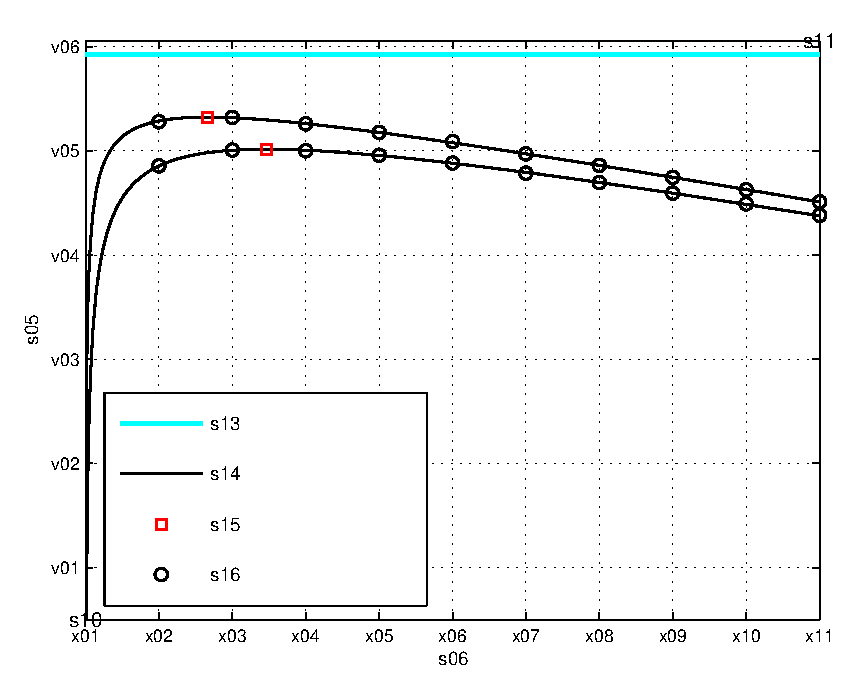
\includegraphics{fig_thr_est_time_tradeoff_AWGN.eps}}%
%\end{psfrags}%
%
% End fig_thr_est_time_tradeoff_AWGN.tex
\end{document}
% See http://www.mathworks.de/matlabcentral/fileexchange/loadFile.do?objectId=4638
% for recent versions of laprint.m.
%
% created by:           LaPrint version 3.16 (13.9.2004)
% created on:           08-Jan-2016 12:22:27
% eps bounding box:     16 cm x 12 cm
% comment:              
%
%\begin{psfrags}%
%\psfragscanon%
%
% text strings:
\psfrag{s05}[b][b]{\fontsize{8.5}{12.75}\fontseries{m}\mathversion{normal}\fontshape{n}\selectfont \color[rgb]{0,0,0}\setlength{\tabcolsep}{0pt}\begin{tabular}{c}$\rs(\tau)$ [bits/sec/Hz]\end{tabular}}%
\psfrag{s06}[t][t]{\fontsize{8.5}{12.75}\fontseries{m}\mathversion{normal}\fontshape{n}\selectfont \color[rgb]{0,0,0}\setlength{\tabcolsep}{0pt}\begin{tabular}{c}$\tau$ [ms]\end{tabular}}%
\psfrag{s10}[][]{\fontsize{10}{15}\fontseries{m}\mathversion{normal}\fontshape{n}\selectfont \color[rgb]{0,0,0}\setlength{\tabcolsep}{0pt}\begin{tabular}{c} \end{tabular}}%
\psfrag{s11}[][]{\fontsize{10}{15}\fontseries{m}\mathversion{normal}\fontshape{n}\selectfont \color[rgb]{0,0,0}\setlength{\tabcolsep}{0pt}\begin{tabular}{c} \end{tabular}}%
\psfrag{s12}[l][l]{\fontsize{8.5}{12.75}\fontseries{m}\mathversion{normal}\fontshape{n}\selectfont \color[rgb]{0,0,0}Simulated}%
\psfrag{s13}[l][l]{\fontsize{8.5}{12.75}\fontseries{m}\mathversion{normal}\fontshape{n}\selectfont \color[rgb]{0,0,0}IM}%
\psfrag{s14}[l][l]{\fontsize{8.5}{12.75}\fontseries{m}\mathversion{normal}\fontshape{n}\selectfont \color[rgb]{0,0,0}EM}%
\psfrag{s15}[l][l]{\fontsize{8.5}{12.75}\fontseries{m}\mathversion{normal}\fontshape{n}\selectfont \color[rgb]{0,0,0}$\trs(\ttau)$}%
\psfrag{s16}[l][l]{\fontsize{8.5}{12.75}\fontseries{m}\mathversion{normal}\fontshape{n}\selectfont \color[rgb]{0,0,0}Simulated}%
%
% axes font properties:
\fontsize{8.5}{12.75}\fontseries{m}\mathversion{normal}%
\fontshape{n}\selectfont%
%
% xticklabels:
\psfrag{x01}[t][t]{0}%
\psfrag{x02}[t][t]{1}%
\psfrag{x03}[t][t]{2}%
\psfrag{x04}[t][t]{3}%
\psfrag{x05}[t][t]{4}%
\psfrag{x06}[t][t]{5}%
\psfrag{x07}[t][t]{6}%
\psfrag{x08}[t][t]{7}%
\psfrag{x09}[t][t]{8}%
\psfrag{x10}[t][t]{9}%
\psfrag{x11}[t][t]{10}%
%
% yticklabels:
\psfrag{v01}[r][r]{1.6}%
\psfrag{v02}[r][r]{1.8}%
\psfrag{v03}[r][r]{2}%
\psfrag{v04}[r][r]{2.2}%
\psfrag{v05}[r][r]{2.4}%
\psfrag{v06}[r][r]{2.6}%
%
% Figure:
%\resizebox{8cm}{!}{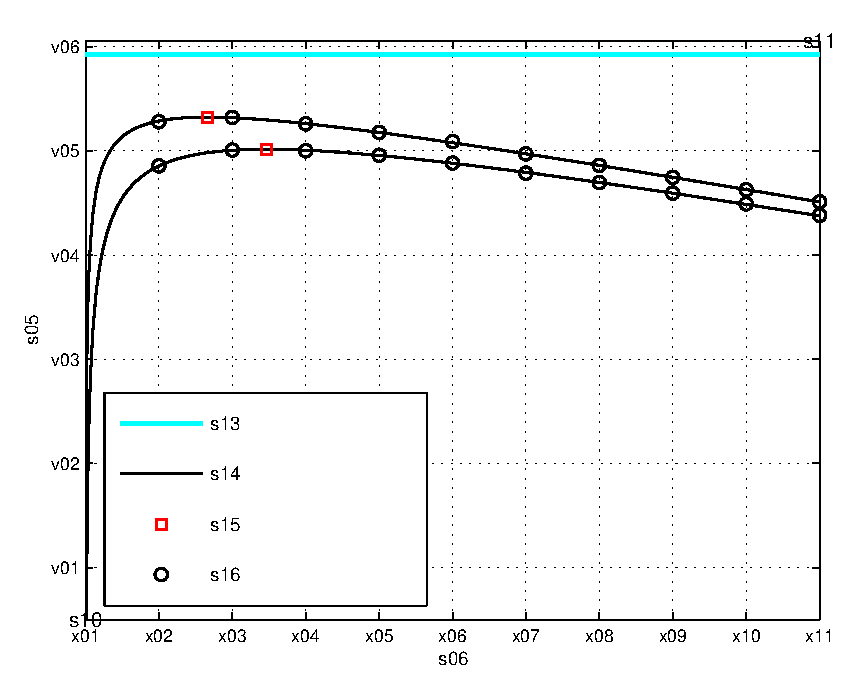
\includegraphics{fig_thr_est_time_tradeoff_AWGN.eps}}%
%\end{psfrags}%
%
% End fig_thr_est_time_tradeoff_AWGN.tex

			\centering
             	        \resizebox{.95 \columnwidth}{!}{%
                        \begin{tikzpicture}[scale=1]
				\node[anchor=south west,inner sep=0] (image) at (0,0)
				{
				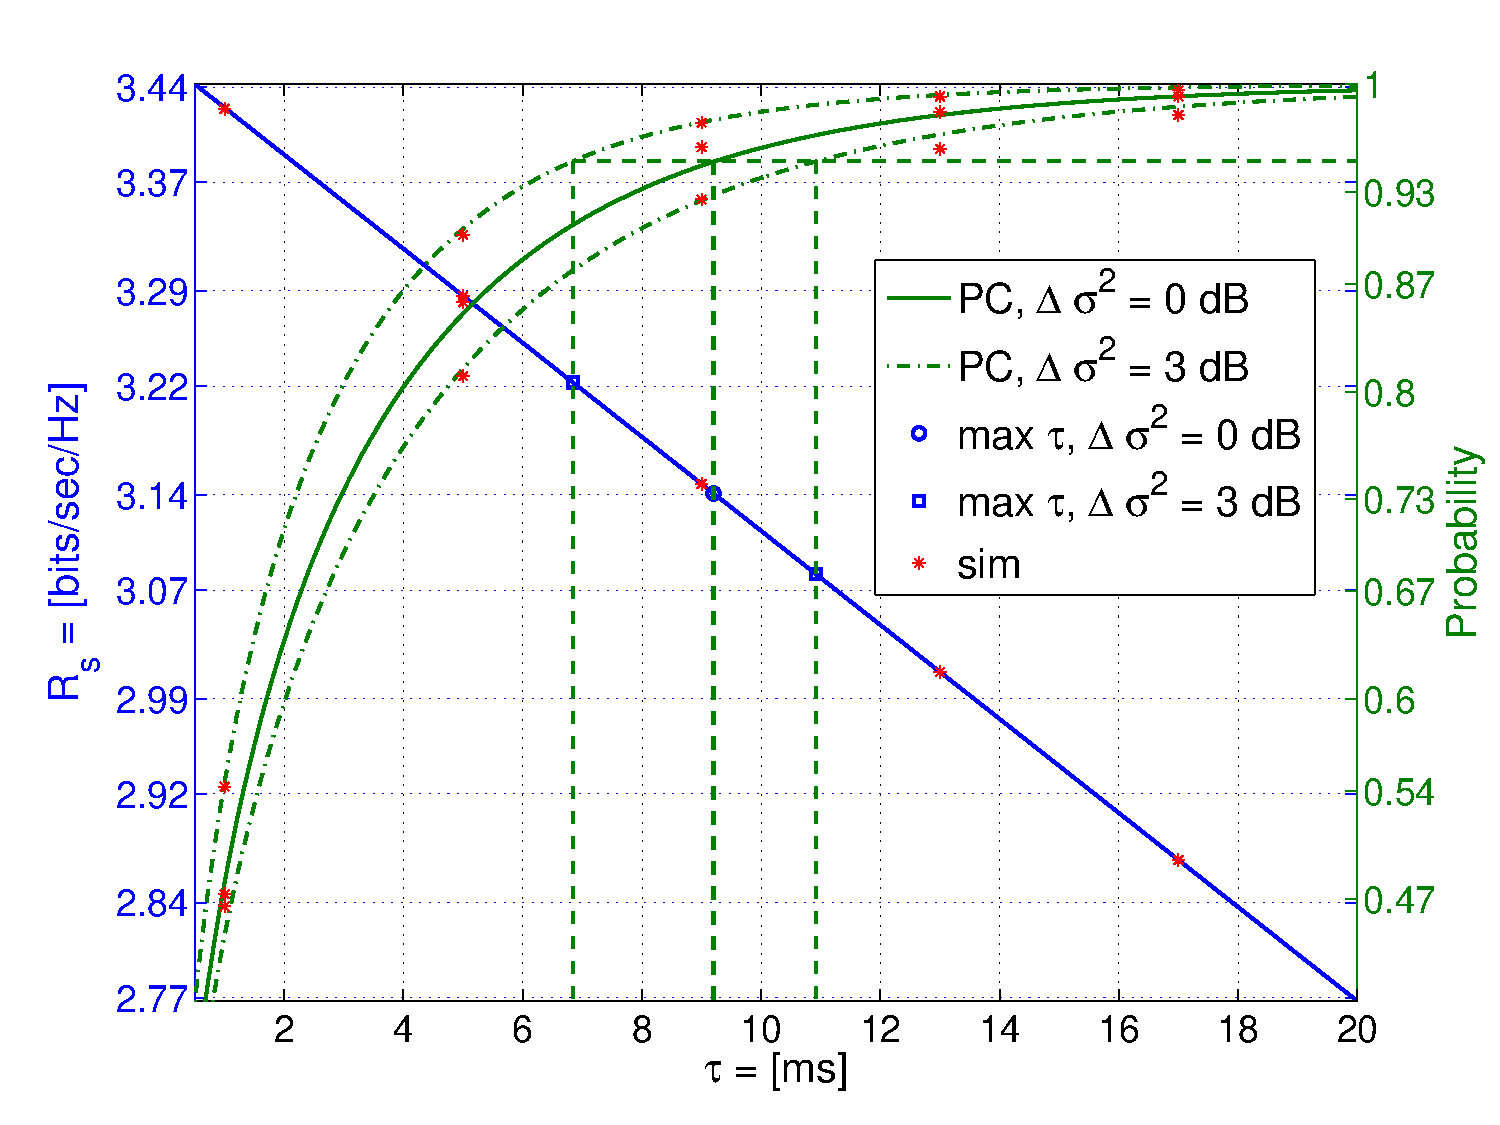
\includegraphics[width= 1.2 \columnwidth]{../kapitel04/figures/fig_thr_est_time_tradeoff_AWGN}
};
				\begin{scope}[x={(image.south east)},y={(image.north west)}]

				\draw (0.38,0.78) arc(-130:130:0.005 and 0.015);
				\node[draw, fill=gray!10,font=\scriptsize] at (0.39,0.735) {$\opc = 0.01$};

				\draw (0.65,0.77) arc(-130:130:0.005 and 0.015);
				\node[draw,fill=gray!10,font=\scriptsize] at (0.66,0.838) {$\opc = 0.1$};
				\node[draw=none,fill=kit-green30, minimum height = 0.6cm, align = center, font = \footnotesize] at (0.5, 1.05) {Estimation-throughput tradeoff};

				%\draw[help lines,xstep=.1,ystep=.1] (0,0) grid (1,1);
				%\foreach \x in {0,1,...,9} { \node [anchor=north] at (\x/10,0) {0.\x}; }
				%\foreach \y in {0,1,...,9} { \node [anchor=east] at (0,\y/10) {0.\y}; }
			\end{scope}
			\end{tikzpicture}
                }
		\end{center}
		\end{column}
	\end{columns}
	\begin{block}{}%{\scriptsize Power control} 
		\vspace{-4mm}
		\begin{align*}
			\preg &= 
			\begin{cases} 
				\frac{\ite \ptran}{ \left(\bpo \Gamma^{-1}(\opc, \apo) - \nps  \right)}, & \mbox{for } \preg < \pc \\
				\pc, & \mbox{for } \preg \ge \pc
				\end{cases} \\
				\text{where  } \apo &= \frac{\test \fsam (1 + \snrrcvdu)^2}{2 + 4 \snrrcvdu} \text{ and } \bpo = \frac{\nps (2 + 4 \snrrcvdu)}{\test \fsam (1 + \snrrcvdu)},
			\end{align*}
	\end{block}
\end{frame}

\section{Hybrid System}
%%%%%%%%%%%%%%%%%%%%%%%%%%%%%%%%%%%%%%%%%%%%%%%%%%%%%%%%%%%%%%%%%%%%%%%%%%%%%%%%
\begin{frame}[t]{Hybrid System}
%%%%%%%%%%%%%%%%%%%%%%%%%%%%%%%%%%%%%%%%%%%%%%%%%%%%%%%%%%%%%%%%%%%%%%%%%%%%%%%%
\end{frame}


\section{Hardware Implementation}
%%%%%%%%%%%%%%%%%%%%%%%%%%%%%%%%%%%%%%%%%%%%%%%%%%%%%%%%%%%%%%%%%%%%%%%%%%%%%%%%
\begin{frame}[t]{Hardware Implementation}
%%%%%%%%%%%%%%%%%%%%%%%%%%%%%%%%%%%%%%%%%%%%%%%%%%%%%%%%%%%%%%%%%%%%%%%%%%%%%%%%
\end{frame}

\subsection{Validation}
%%%%%%%%%%%%%%%%%%%%%%%%%%%%%%%%%%%%%%%%%%%%%%%%%%%%%%%%%%%%%%%%%%%%%%%%%%%%%%%%
\begin{frame}[t]{Validation}
%%%%%%%%%%%%%%%%%%%%%%%%%%%%%%%%%%%%%%%%%%%%%%%%%%%%%%%%%%%%%%%%%%%%%%%%%%%%%%%%
\end{frame}

\subsection{Demonstration}
%%%%%%%%%%%%%%%%%%%%%%%%%%%%%%%%%%%%%%%%%%%%%%%%%%%%%%%%%%%%%%%%%%%%%%%%%%%%%%%%
\begin{frame}[t]{Demonstration}
%%%%%%%%%%%%%%%%%%%%%%%%%%%%%%%%%%%%%%%%%%%%%%%%%%%%%%%%%%%%%%%%%%%%%%%%%%%%%%%%
\end{frame}

\section{Conclusion}
%%%%%%%%%%%%%%%%%%%%%%%%%%%%%%%%%%%%%%%%%%%%%%%%%%%%%%%%%%%%%%%%%%%%%%%%%%%%%%%%
\begin{frame}[t]{Conclusion}
%%%%%%%%%%%%%%%%%%%%%%%%%%%%%%%%%%%%%%%%%%%%%%%%%%%%%%%%%%%%%%%%%%%%%%%%%%%%%%%%
\end{frame}

%%%%%%%%%%%%%%%%%%%%%%%%%%%%%%%%%%%%%%%%%%%%%%%%%%%%%%%%%%%%%%%%%%%%%%%%%%%%%%%%
\begin{frame}[c]{}
%%%%%%%%%%%%%%%%%%%%%%%%%%%%%%%%%%%%%%%%%%%%%%%%%%%%%%%%%%%%%%%%%%%%%%%%%%%%%%%%
\begin{center}
Thank you for your Attention!
\end{center}
\end{frame}

\end{document}	
